% layout and global options
\documentclass
[
  draft    = true,
  fontsize = 11pt,
  parskip  = half-,
  BCOR     = 0pt,
  DIV      = 11,
  ngerman,
  dvipsnames
]
{scrartcl}

% default packages
\usepackage[utf8]{inputenc}
\usepackage[T1]{fontenc}
\usepackage{lmodern}
\usepackage{babel}
% extra packages
\usepackage{amsmath}
\usepackage{amssymb}
\usepackage{enumerate}
\usepackage{graphicx}
\usepackage{ifthen}
\usepackage{siunitx}
\usepackage{tikz}
\usepackage{url}

% basic calculations in TikZ
\usetikzlibrary{calc}

% use comma as decimal separator
\sisetup{locale=DE, group-minimum-digits=4}

% no header no footer
\pagestyle{empty}

% ------------------------------------------------------------------------------
\begin{document}
% ------------------------------------------------------------------------------

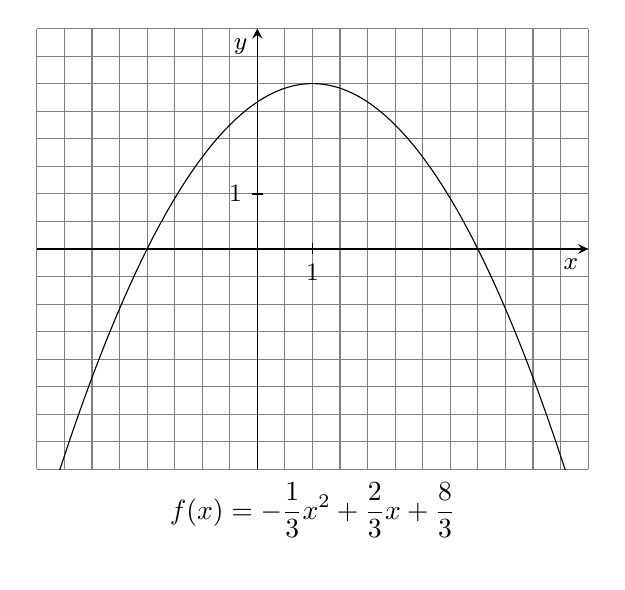
\begin{tikzpicture}[scale=0.7]
  % grid
  \draw[draw=black!50!white] (-4.000, -4.000) grid[step=0.5] (6.000, 4.000);
  % x-axis
  \draw[line width=0.6pt, ->, >=stealth] (-4.000, 0) -- (6.000, 0) node[below left] {\small$x$};
  % x scale
  \draw[line width=0.6pt] (1, 0.1) -- (1, -0.1) node[below] {\small1};
  % y-axis
  \draw[line width=0.6pt, ->, >=stealth] (0, -4.000) -- (0, 4.000) node[below left] {\small$y$};
  % y scale
  \draw[line width=0.6pt] (0.1, 1) -- (-0.1, 1) node[left] {\small1};
  % function
  \begin{scope}
    \clip (-4.000, -4.000) rectangle (6.000, 4.000);
    \draw plot[smooth] coordinates
    {
      ( -4.000,  -5.000) ( -3.900,  -5.000) ( -3.800,  -4.680)
      ( -3.700,  -4.363) ( -3.600,  -4.053) ( -3.500,  -3.750)
      ( -3.400,  -3.453) ( -3.300,  -3.163) ( -3.200,  -2.880)
      ( -3.100,  -2.603) ( -3.000,  -2.333) ( -2.900,  -2.070)
      ( -2.800,  -1.813) ( -2.700,  -1.563) ( -2.600,  -1.320)
      ( -2.500,  -1.083) ( -2.400,  -0.853) ( -2.300,  -0.630)
      ( -2.200,  -0.413) ( -2.100,  -0.203) ( -2.000,   0.000)
      ( -1.900,   0.197) ( -1.800,   0.387) ( -1.700,   0.570)
      ( -1.600,   0.747) ( -1.500,   0.917) ( -1.400,   1.080)
      ( -1.300,   1.237) ( -1.200,   1.387) ( -1.100,   1.530)
      ( -1.000,   1.667) ( -0.900,   1.797) ( -0.800,   1.920)
      ( -0.700,   2.037) ( -0.600,   2.147) ( -0.500,   2.250)
      ( -0.400,   2.347) ( -0.300,   2.437) ( -0.200,   2.520)
      ( -0.100,   2.597) (  0.000,   2.667) (  0.100,   2.730)
      (  0.200,   2.787) (  0.300,   2.837) (  0.400,   2.880)
      (  0.500,   2.917) (  0.600,   2.947) (  0.700,   2.970)
      (  0.800,   2.987) (  0.900,   2.997) (  1.000,   3.000)
      (  1.100,   2.997) (  1.200,   2.987) (  1.300,   2.970)
      (  1.400,   2.947) (  1.500,   2.917) (  1.600,   2.880)
      (  1.700,   2.837) (  1.800,   2.787) (  1.900,   2.730)
      (  2.000,   2.667) (  2.100,   2.597) (  2.200,   2.520)
      (  2.300,   2.437) (  2.400,   2.347) (  2.500,   2.250)
      (  2.600,   2.147) (  2.700,   2.037) (  2.800,   1.920)
      (  2.900,   1.797) (  3.000,   1.667) (  3.100,   1.530)
      (  3.200,   1.387) (  3.300,   1.237) (  3.400,   1.080)
      (  3.500,   0.917) (  3.600,   0.747) (  3.700,   0.570)
      (  3.800,   0.387) (  3.900,   0.197) (  4.000,   0.000)
      (  4.100,  -0.203) (  4.200,  -0.413) (  4.300,  -0.630)
      (  4.400,  -0.853) (  4.500,  -1.083) (  4.600,  -1.320)
      (  4.700,  -1.563) (  4.800,  -1.813) (  4.900,  -2.070)
      (  5.000,  -2.333) (  5.100,  -2.603) (  5.200,  -2.880)
      (  5.300,  -3.163) (  5.400,  -3.453) (  5.500,  -3.750)
      (  5.600,  -4.053) (  5.700,  -4.363) (  5.800,  -4.680)
      (  5.900,  -5.000) (  6.000,  -5.000)
    };
  \end{scope}
  \node[below] at (1.000, -4.000)
  {%
    \rule[-1.1\baselineskip]{0pt}{2.2\baselineskip}%
    \begin{minipage}{7.000cm}%
      \begin{equation*}%
        f(x)=-\frac{1}{3}x^2+\frac{2}{3}x+\frac{8}{3}
      \end{equation*}%
    \end{minipage}%
  };
\end{tikzpicture}

\hfill
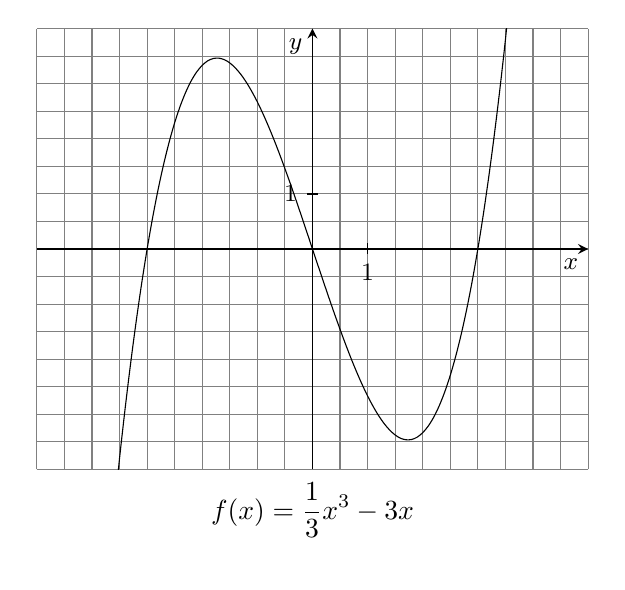
\begin{tikzpicture}[scale=0.7]
  % grid
  \draw[draw=black!50!white] (-5.000, -4.000) grid[step=0.5] (5.000, 4.000);
  % x-axis
  \draw[line width=0.6pt, ->, >=stealth] (-5.000, 0) -- (5.000, 0) node[below left] {\small$x$};
  % x scale
  \draw[line width=0.6pt] (1, 0.1) -- (1, -0.1) node[below] {\small1};
  % y-axis
  \draw[line width=0.6pt, ->, >=stealth] (0, -4.000) -- (0, 4.000) node[below left] {\small$y$};
  % y scale
  \draw[line width=0.6pt] (0.1, 1) -- (-0.1, 1) node[left] {\small1};
  % function
  \begin{scope}
    \clip (-5.000, -4.000) rectangle (5.000, 4.000);
    \draw plot[smooth] coordinates
    {
      ( -5.000,  -5.000) ( -4.900,  -5.000) ( -4.800,  -5.000)
      ( -4.700,  -5.000) ( -4.600,  -5.000) ( -4.500,  -5.000)
      ( -4.400,  -5.000) ( -4.300,  -5.000) ( -4.200,  -5.000)
      ( -4.100,  -5.000) ( -4.000,  -5.000) ( -3.900,  -5.000)
      ( -3.800,  -5.000) ( -3.700,  -5.000) ( -3.600,  -4.752)
      ( -3.500,  -3.792) ( -3.400,  -2.901) ( -3.300,  -2.079)
      ( -3.200,  -1.323) ( -3.100,  -0.630) ( -3.000,   0.000)
      ( -2.900,   0.570) ( -2.800,   1.083) ( -2.700,   1.539)
      ( -2.600,   1.941) ( -2.500,   2.292) ( -2.400,   2.592)
      ( -2.300,   2.844) ( -2.200,   3.051) ( -2.100,   3.213)
      ( -2.000,   3.333) ( -1.900,   3.414) ( -1.800,   3.456)
      ( -1.700,   3.462) ( -1.600,   3.435) ( -1.500,   3.375)
      ( -1.400,   3.285) ( -1.300,   3.168) ( -1.200,   3.024)
      ( -1.100,   2.856) ( -1.000,   2.667) ( -0.900,   2.457)
      ( -0.800,   2.229) ( -0.700,   1.986) ( -0.600,   1.728)
      ( -0.500,   1.458) ( -0.400,   1.179) ( -0.300,   0.891)
      ( -0.200,   0.597) ( -0.100,   0.300) (  0.000,   0.000)
      (  0.100,  -0.300) (  0.200,  -0.597) (  0.300,  -0.891)
      (  0.400,  -1.179) (  0.500,  -1.458) (  0.600,  -1.728)
      (  0.700,  -1.986) (  0.800,  -2.229) (  0.900,  -2.457)
      (  1.000,  -2.667) (  1.100,  -2.856) (  1.200,  -3.024)
      (  1.300,  -3.168) (  1.400,  -3.285) (  1.500,  -3.375)
      (  1.600,  -3.435) (  1.700,  -3.462) (  1.800,  -3.456)
      (  1.900,  -3.414) (  2.000,  -3.333) (  2.100,  -3.213)
      (  2.200,  -3.051) (  2.300,  -2.844) (  2.400,  -2.592)
      (  2.500,  -2.292) (  2.600,  -1.941) (  2.700,  -1.539)
      (  2.800,  -1.083) (  2.900,  -0.570) (  3.000,   0.000)
      (  3.100,   0.630) (  3.200,   1.323) (  3.300,   2.079)
      (  3.400,   2.901) (  3.500,   3.792) (  3.600,   4.752)
      (  3.700,   5.000) (  3.800,   5.000) (  3.900,   5.000)
      (  4.000,   5.000) (  4.100,   5.000) (  4.200,   5.000)
      (  4.300,   5.000) (  4.400,   5.000) (  4.500,   5.000)
      (  4.600,   5.000) (  4.700,   5.000) (  4.800,   5.000)
      (  4.900,   5.000) (  5.000,   5.000)
    };
  \end{scope}
  \node[below] at (0.000, -4.000)
  {%
    \rule[-1.1\baselineskip]{0pt}{2.2\baselineskip}%
    \begin{minipage}{7.000cm}%
      \begin{equation*}%
        f(x)=\frac{1}{3}x^3-3x
      \end{equation*}%
    \end{minipage}%
  };
\end{tikzpicture}


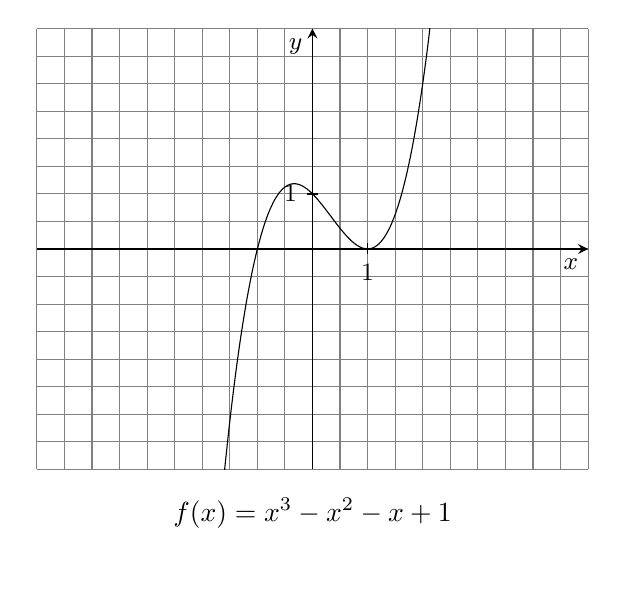
\begin{tikzpicture}[scale=0.7]
  % grid
  \draw[draw=black!50!white] (-5.000, -4.000) grid[step=0.5] (5.000, 4.000);
  % x-axis
  \draw[line width=0.6pt, ->, >=stealth] (-5.000, 0) -- (5.000, 0) node[below left] {\small$x$};
  % x scale
  \draw[line width=0.6pt] (1, 0.1) -- (1, -0.1) node[below] {\small1};
  % y-axis
  \draw[line width=0.6pt, ->, >=stealth] (0, -4.000) -- (0, 4.000) node[below left] {\small$y$};
  % y scale
  \draw[line width=0.6pt] (0.1, 1) -- (-0.1, 1) node[left] {\small1};
  % function
  \begin{scope}
    \clip (-5.000, -4.000) rectangle (5.000, 4.000);
    \draw plot[smooth] coordinates
    {
      ( -5.000,  -5.000) ( -4.900,  -5.000) ( -4.800,  -5.000)
      ( -4.700,  -5.000) ( -4.600,  -5.000) ( -4.500,  -5.000)
      ( -4.400,  -5.000) ( -4.300,  -5.000) ( -4.200,  -5.000)
      ( -4.100,  -5.000) ( -4.000,  -5.000) ( -3.900,  -5.000)
      ( -3.800,  -5.000) ( -3.700,  -5.000) ( -3.600,  -5.000)
      ( -3.500,  -5.000) ( -3.400,  -5.000) ( -3.300,  -5.000)
      ( -3.200,  -5.000) ( -3.100,  -5.000) ( -3.000,  -5.000)
      ( -2.900,  -5.000) ( -2.800,  -5.000) ( -2.700,  -5.000)
      ( -2.600,  -5.000) ( -2.500,  -5.000) ( -2.400,  -5.000)
      ( -2.300,  -5.000) ( -2.200,  -5.000) ( -2.100,  -5.000)
      ( -2.000,  -5.000) ( -1.900,  -5.000) ( -1.800,  -5.000)
      ( -1.700,  -5.000) ( -1.600,  -4.056) ( -1.500,  -3.125)
      ( -1.400,  -2.304) ( -1.300,  -1.587) ( -1.200,  -0.968)
      ( -1.100,  -0.441) ( -1.000,   0.000) ( -0.900,   0.361)
      ( -0.800,   0.648) ( -0.700,   0.867) ( -0.600,   1.024)
      ( -0.500,   1.125) ( -0.400,   1.176) ( -0.300,   1.183)
      ( -0.200,   1.152) ( -0.100,   1.089) (  0.000,   1.000)
      (  0.100,   0.891) (  0.200,   0.768) (  0.300,   0.637)
      (  0.400,   0.504) (  0.500,   0.375) (  0.600,   0.256)
      (  0.700,   0.153) (  0.800,   0.072) (  0.900,   0.019)
      (  1.000,   0.000) (  1.100,   0.021) (  1.200,   0.088)
      (  1.300,   0.207) (  1.400,   0.384) (  1.500,   0.625)
      (  1.600,   0.936) (  1.700,   1.323) (  1.800,   1.792)
      (  1.900,   2.349) (  2.000,   3.000) (  2.100,   3.751)
      (  2.200,   4.608) (  2.300,   5.000) (  2.400,   5.000)
      (  2.500,   5.000) (  2.600,   5.000) (  2.700,   5.000)
      (  2.800,   5.000) (  2.900,   5.000) (  3.000,   5.000)
      (  3.100,   5.000) (  3.200,   5.000) (  3.300,   5.000)
      (  3.400,   5.000) (  3.500,   5.000) (  3.600,   5.000)
      (  3.700,   5.000) (  3.800,   5.000) (  3.900,   5.000)
      (  4.000,   5.000) (  4.100,   5.000) (  4.200,   5.000)
      (  4.300,   5.000) (  4.400,   5.000) (  4.500,   5.000)
      (  4.600,   5.000) (  4.700,   5.000) (  4.800,   5.000)
      (  4.900,   5.000) (  5.000,   5.000)
    };
  \end{scope}
  \node[below] at (0.000, -4.000)
  {%
    \rule[-1.1\baselineskip]{0pt}{2.2\baselineskip}%
    \begin{minipage}{7.000cm}%
      \begin{equation*}%
        f(x)=x^3-x^2-x+1
      \end{equation*}%
    \end{minipage}%
  };
\end{tikzpicture}

\hfill
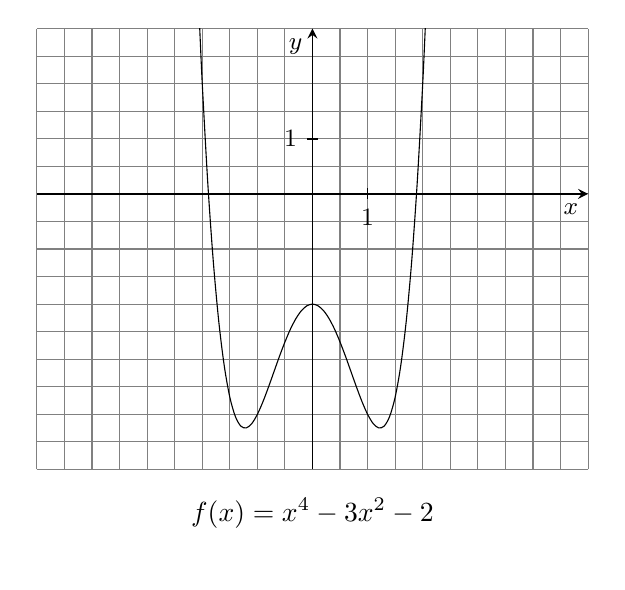
\begin{tikzpicture}[scale=0.7]
  % grid
  \draw[draw=black!50!white] (-5.000, -5.000) grid[step=0.5] (5.000, 3.000);
  % x-axis
  \draw[line width=0.6pt, ->, >=stealth] (-5.000, 0) -- (5.000, 0) node[below left] {\small$x$};
  % x scale
  \draw[line width=0.6pt] (1, 0.1) -- (1, -0.1) node[below] {\small1};
  % y-axis
  \draw[line width=0.6pt, ->, >=stealth] (0, -5.000) -- (0, 3.000) node[below left] {\small$y$};
  % y scale
  \draw[line width=0.6pt] (0.1, 1) -- (-0.1, 1) node[left] {\small1};
  % function
  \begin{scope}
    \clip (-5.000, -5.000) rectangle (5.000, 3.000);
    \draw plot[smooth] coordinates
    {
      ( -5.000,   4.000) ( -4.900,   4.000) ( -4.800,   4.000)
      ( -4.700,   4.000) ( -4.600,   4.000) ( -4.500,   4.000)
      ( -4.400,   4.000) ( -4.300,   4.000) ( -4.200,   4.000)
      ( -4.100,   4.000) ( -4.000,   4.000) ( -3.900,   4.000)
      ( -3.800,   4.000) ( -3.700,   4.000) ( -3.600,   4.000)
      ( -3.500,   4.000) ( -3.400,   4.000) ( -3.300,   4.000)
      ( -3.200,   4.000) ( -3.100,   4.000) ( -3.000,   4.000)
      ( -2.900,   4.000) ( -2.800,   4.000) ( -2.700,   4.000)
      ( -2.600,   4.000) ( -2.500,   4.000) ( -2.400,   4.000)
      ( -2.300,   4.000) ( -2.200,   4.000) ( -2.100,   4.000)
      ( -2.000,   2.000) ( -1.900,   0.202) ( -1.800,  -1.222)
      ( -1.700,  -2.318) ( -1.600,  -3.126) ( -1.500,  -3.688)
      ( -1.400,  -4.038) ( -1.300,  -4.214) ( -1.200,  -4.246)
      ( -1.100,  -4.166) ( -1.000,  -4.000) ( -0.900,  -3.774)
      ( -0.800,  -3.510) ( -0.700,  -3.230) ( -0.600,  -2.950)
      ( -0.500,  -2.688) ( -0.400,  -2.454) ( -0.300,  -2.262)
      ( -0.200,  -2.118) ( -0.100,  -2.030) (  0.000,  -2.000)
      (  0.100,  -2.030) (  0.200,  -2.118) (  0.300,  -2.262)
      (  0.400,  -2.454) (  0.500,  -2.688) (  0.600,  -2.950)
      (  0.700,  -3.230) (  0.800,  -3.510) (  0.900,  -3.774)
      (  1.000,  -4.000) (  1.100,  -4.166) (  1.200,  -4.246)
      (  1.300,  -4.214) (  1.400,  -4.038) (  1.500,  -3.688)
      (  1.600,  -3.126) (  1.700,  -2.318) (  1.800,  -1.222)
      (  1.900,   0.202) (  2.000,   2.000) (  2.100,   4.000)
      (  2.200,   4.000) (  2.300,   4.000) (  2.400,   4.000)
      (  2.500,   4.000) (  2.600,   4.000) (  2.700,   4.000)
      (  2.800,   4.000) (  2.900,   4.000) (  3.000,   4.000)
      (  3.100,   4.000) (  3.200,   4.000) (  3.300,   4.000)
      (  3.400,   4.000) (  3.500,   4.000) (  3.600,   4.000)
      (  3.700,   4.000) (  3.800,   4.000) (  3.900,   4.000)
      (  4.000,   4.000) (  4.100,   4.000) (  4.200,   4.000)
      (  4.300,   4.000) (  4.400,   4.000) (  4.500,   4.000)
      (  4.600,   4.000) (  4.700,   4.000) (  4.800,   4.000)
      (  4.900,   4.000) (  5.000,   4.000)
    };
  \end{scope}
  \node[below] at (0.000, -5.000)
  {%
    \rule[-1.1\baselineskip]{0pt}{2.2\baselineskip}%
    \begin{minipage}{7.000cm}%
      \begin{equation*}%
        f(x)=x^4-3x^2-2
      \end{equation*}%
    \end{minipage}%
  };
\end{tikzpicture}


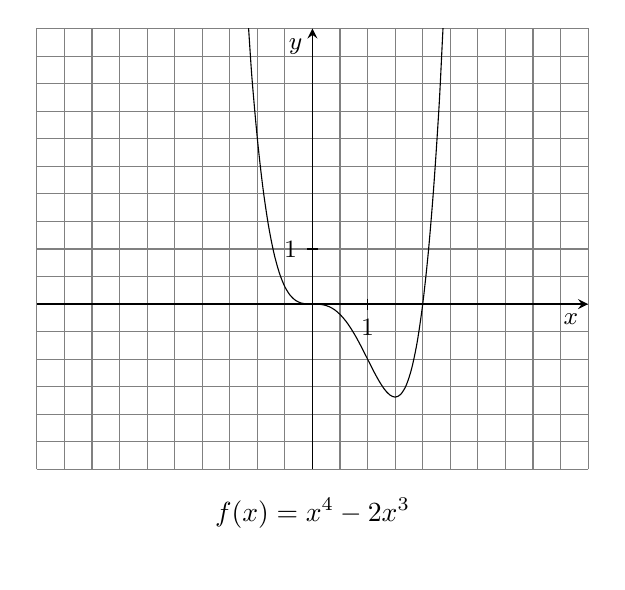
\begin{tikzpicture}[scale=0.7]
  % grid
  \draw[draw=black!50!white] (-5.000, -3.000) grid[step=0.5] (5.000, 5.000);
  % x-axis
  \draw[line width=0.6pt, ->, >=stealth] (-5.000, 0) -- (5.000, 0) node[below left] {\small$x$};
  % x scale
  \draw[line width=0.6pt] (1, 0.1) -- (1, -0.1) node[below] {\small1};
  % y-axis
  \draw[line width=0.6pt, ->, >=stealth] (0, -3.000) -- (0, 5.000) node[below left] {\small$y$};
  % y scale
  \draw[line width=0.6pt] (0.1, 1) -- (-0.1, 1) node[left] {\small1};
  % function
  \begin{scope}
    \clip (-5.000, -3.000) rectangle (5.000, 5.000);
    \draw plot[smooth] coordinates
    {
      ( -5.000,   6.000) ( -4.900,   6.000) ( -4.800,   6.000)
      ( -4.700,   6.000) ( -4.600,   6.000) ( -4.500,   6.000)
      ( -4.400,   6.000) ( -4.300,   6.000) ( -4.200,   6.000)
      ( -4.100,   6.000) ( -4.000,   6.000) ( -3.900,   6.000)
      ( -3.800,   6.000) ( -3.700,   6.000) ( -3.600,   6.000)
      ( -3.500,   6.000) ( -3.400,   6.000) ( -3.300,   6.000)
      ( -3.200,   6.000) ( -3.100,   6.000) ( -3.000,   6.000)
      ( -2.900,   6.000) ( -2.800,   6.000) ( -2.700,   6.000)
      ( -2.600,   6.000) ( -2.500,   6.000) ( -2.400,   6.000)
      ( -2.300,   6.000) ( -2.200,   6.000) ( -2.100,   6.000)
      ( -2.000,   6.000) ( -1.900,   6.000) ( -1.800,   6.000)
      ( -1.700,   6.000) ( -1.600,   6.000) ( -1.500,   6.000)
      ( -1.400,   6.000) ( -1.300,   6.000) ( -1.200,   5.530)
      ( -1.100,   4.126) ( -1.000,   3.000) ( -0.900,   2.114)
      ( -0.800,   1.434) ( -0.700,   0.926) ( -0.600,   0.562)
      ( -0.500,   0.312) ( -0.400,   0.154) ( -0.300,   0.062)
      ( -0.200,   0.018) ( -0.100,   0.002) (  0.000,   0.000)
      (  0.100,  -0.002) (  0.200,  -0.014) (  0.300,  -0.046)
      (  0.400,  -0.102) (  0.500,  -0.188) (  0.600,  -0.302)
      (  0.700,  -0.446) (  0.800,  -0.614) (  0.900,  -0.802)
      (  1.000,  -1.000) (  1.100,  -1.198) (  1.200,  -1.382)
      (  1.300,  -1.538) (  1.400,  -1.646) (  1.500,  -1.688)
      (  1.600,  -1.638) (  1.700,  -1.474) (  1.800,  -1.166)
      (  1.900,  -0.686) (  2.000,   0.000) (  2.100,   0.926)
      (  2.200,   2.130) (  2.300,   3.650) (  2.400,   5.530)
      (  2.500,   6.000) (  2.600,   6.000) (  2.700,   6.000)
      (  2.800,   6.000) (  2.900,   6.000) (  3.000,   6.000)
      (  3.100,   6.000) (  3.200,   6.000) (  3.300,   6.000)
      (  3.400,   6.000) (  3.500,   6.000) (  3.600,   6.000)
      (  3.700,   6.000) (  3.800,   6.000) (  3.900,   6.000)
      (  4.000,   6.000) (  4.100,   6.000) (  4.200,   6.000)
      (  4.300,   6.000) (  4.400,   6.000) (  4.500,   6.000)
      (  4.600,   6.000) (  4.700,   6.000) (  4.800,   6.000)
      (  4.900,   6.000) (  5.000,   6.000)
    };
  \end{scope}
  \node[below] at (0.000, -3.000)
  {%
    \rule[-1.1\baselineskip]{0pt}{2.2\baselineskip}%
    \begin{minipage}{7.000cm}%
      \begin{equation*}%
        f(x)=x^4-2x^3
      \end{equation*}%
    \end{minipage}%
  };
\end{tikzpicture}

\hfill
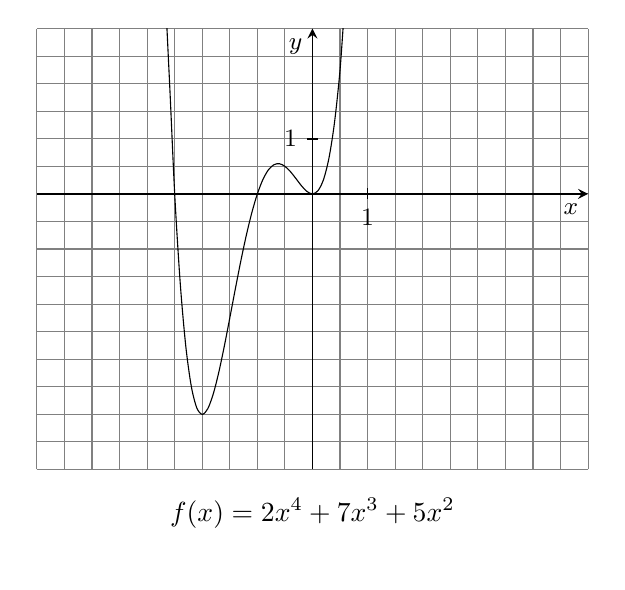
\begin{tikzpicture}[scale=0.7]
  % grid
  \draw[draw=black!50!white] (-5.000, -5.000) grid[step=0.5] (5.000, 3.000);
  % x-axis
  \draw[line width=0.6pt, ->, >=stealth] (-5.000, 0) -- (5.000, 0) node[below left] {\small$x$};
  % x scale
  \draw[line width=0.6pt] (1, 0.1) -- (1, -0.1) node[below] {\small1};
  % y-axis
  \draw[line width=0.6pt, ->, >=stealth] (0, -5.000) -- (0, 3.000) node[below left] {\small$y$};
  % y scale
  \draw[line width=0.6pt] (0.1, 1) -- (-0.1, 1) node[left] {\small1};
  % function
  \begin{scope}
    \clip (-5.000, -5.000) rectangle (5.000, 3.000);
    \draw plot[smooth] coordinates
    {
      ( -5.000,   4.000) ( -4.900,   4.000) ( -4.800,   4.000)
      ( -4.700,   4.000) ( -4.600,   4.000) ( -4.500,   4.000)
      ( -4.400,   4.000) ( -4.300,   4.000) ( -4.200,   4.000)
      ( -4.100,   4.000) ( -4.000,   4.000) ( -3.900,   4.000)
      ( -3.800,   4.000) ( -3.700,   4.000) ( -3.600,   4.000)
      ( -3.500,   4.000) ( -3.400,   4.000) ( -3.300,   4.000)
      ( -3.200,   4.000) ( -3.100,   4.000) ( -3.000,   4.000)
      ( -2.900,   4.000) ( -2.800,   4.000) ( -2.700,   4.000)
      ( -2.600,   2.163) ( -2.500,   0.000) ( -2.400,  -1.613)
      ( -2.300,  -2.751) ( -2.200,  -3.485) ( -2.100,  -3.881)
      ( -2.000,  -4.000) ( -1.900,  -3.899) ( -1.800,  -3.629)
      ( -1.700,  -3.237) ( -1.600,  -2.765) ( -1.500,  -2.250)
      ( -1.400,  -1.725) ( -1.300,  -1.217) ( -1.200,  -0.749)
      ( -1.100,  -0.339) ( -1.000,   0.000) ( -0.900,   0.259)
      ( -0.800,   0.435) ( -0.700,   0.529) ( -0.600,   0.547)
      ( -0.500,   0.500) ( -0.400,   0.403) ( -0.300,   0.277)
      ( -0.200,   0.147) ( -0.100,   0.043) (  0.000,   0.000)
      (  0.100,   0.057) (  0.200,   0.259) (  0.300,   0.655)
      (  0.400,   1.299) (  0.500,   2.250) (  0.600,   3.571)
      (  0.700,   4.000) (  0.800,   4.000) (  0.900,   4.000)
      (  1.000,   4.000) (  1.100,   4.000) (  1.200,   4.000)
      (  1.300,   4.000) (  1.400,   4.000) (  1.500,   4.000)
      (  1.600,   4.000) (  1.700,   4.000) (  1.800,   4.000)
      (  1.900,   4.000) (  2.000,   4.000) (  2.100,   4.000)
      (  2.200,   4.000) (  2.300,   4.000) (  2.400,   4.000)
      (  2.500,   4.000) (  2.600,   4.000) (  2.700,   4.000)
      (  2.800,   4.000) (  2.900,   4.000) (  3.000,   4.000)
      (  3.100,   4.000) (  3.200,   4.000) (  3.300,   4.000)
      (  3.400,   4.000) (  3.500,   4.000) (  3.600,   4.000)
      (  3.700,   4.000) (  3.800,   4.000) (  3.900,   4.000)
      (  4.000,   4.000) (  4.100,   4.000) (  4.200,   4.000)
      (  4.300,   4.000) (  4.400,   4.000) (  4.500,   4.000)
      (  4.600,   4.000) (  4.700,   4.000) (  4.800,   4.000)
      (  4.900,   4.000) (  5.000,   4.000)
    };
  \end{scope}
  \node[below] at (0.000, -5.000)
  {%
    \rule[-1.1\baselineskip]{0pt}{2.2\baselineskip}%
    \begin{minipage}{7.000cm}%
      \begin{equation*}%
        f(x)=2x^4+7x^3+5x^2
      \end{equation*}%
    \end{minipage}%
  };
\end{tikzpicture}


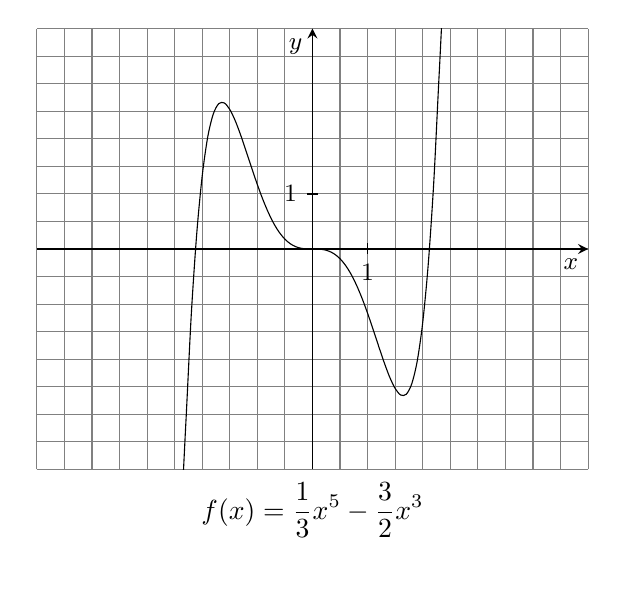
\begin{tikzpicture}[scale=0.7]
  % grid
  \draw[draw=black!50!white] (-5.000, -4.000) grid[step=0.5] (5.000, 4.000);
  % x-axis
  \draw[line width=0.6pt, ->, >=stealth] (-5.000, 0) -- (5.000, 0) node[below left] {\small$x$};
  % x scale
  \draw[line width=0.6pt] (1, 0.1) -- (1, -0.1) node[below] {\small1};
  % y-axis
  \draw[line width=0.6pt, ->, >=stealth] (0, -4.000) -- (0, 4.000) node[below left] {\small$y$};
  % y scale
  \draw[line width=0.6pt] (0.1, 1) -- (-0.1, 1) node[left] {\small1};
  % function
  \begin{scope}
    \clip (-5.000, -4.000) rectangle (5.000, 4.000);
    \draw plot[smooth] coordinates
    {
      ( -5.000,  -5.000) ( -4.900,  -5.000) ( -4.800,  -5.000)
      ( -4.700,  -5.000) ( -4.600,  -5.000) ( -4.500,  -5.000)
      ( -4.400,  -5.000) ( -4.300,  -5.000) ( -4.200,  -5.000)
      ( -4.100,  -5.000) ( -4.000,  -5.000) ( -3.900,  -5.000)
      ( -3.800,  -5.000) ( -3.700,  -5.000) ( -3.600,  -5.000)
      ( -3.500,  -5.000) ( -3.400,  -5.000) ( -3.300,  -5.000)
      ( -3.200,  -5.000) ( -3.100,  -5.000) ( -3.000,  -5.000)
      ( -2.900,  -5.000) ( -2.800,  -5.000) ( -2.700,  -5.000)
      ( -2.600,  -5.000) ( -2.500,  -5.000) ( -2.400,  -5.000)
      ( -2.300,  -3.204) ( -2.200,  -1.207) ( -2.100,   0.278)
      ( -2.000,   1.333) ( -1.900,   2.035) ( -1.800,   2.449)
      ( -1.700,   2.637) ( -1.600,   2.649) ( -1.500,   2.531)
      ( -1.400,   2.323) ( -1.300,   2.058) ( -1.200,   1.763)
      ( -1.100,   1.460) ( -1.000,   1.167) ( -0.900,   0.897)
      ( -0.800,   0.659) ( -0.700,   0.458) ( -0.600,   0.298)
      ( -0.500,   0.177) ( -0.400,   0.093) ( -0.300,   0.040)
      ( -0.200,   0.012) ( -0.100,   0.001) (  0.000,   0.000)
      (  0.100,  -0.001) (  0.200,  -0.012) (  0.300,  -0.040)
      (  0.400,  -0.093) (  0.500,  -0.177) (  0.600,  -0.298)
      (  0.700,  -0.458) (  0.800,  -0.659) (  0.900,  -0.897)
      (  1.000,  -1.167) (  1.100,  -1.460) (  1.200,  -1.763)
      (  1.300,  -2.058) (  1.400,  -2.323) (  1.500,  -2.531)
      (  1.600,  -2.649) (  1.700,  -2.637) (  1.800,  -2.449)
      (  1.900,  -2.035) (  2.000,  -1.333) (  2.100,  -0.278)
      (  2.200,   1.207) (  2.300,   3.204) (  2.400,   5.000)
      (  2.500,   5.000) (  2.600,   5.000) (  2.700,   5.000)
      (  2.800,   5.000) (  2.900,   5.000) (  3.000,   5.000)
      (  3.100,   5.000) (  3.200,   5.000) (  3.300,   5.000)
      (  3.400,   5.000) (  3.500,   5.000) (  3.600,   5.000)
      (  3.700,   5.000) (  3.800,   5.000) (  3.900,   5.000)
      (  4.000,   5.000) (  4.100,   5.000) (  4.200,   5.000)
      (  4.300,   5.000) (  4.400,   5.000) (  4.500,   5.000)
      (  4.600,   5.000) (  4.700,   5.000) (  4.800,   5.000)
      (  4.900,   5.000) (  5.000,   5.000)
    };
  \end{scope}
  \node[below] at (0.000, -4.000)
  {%
    \rule[-1.1\baselineskip]{0pt}{2.2\baselineskip}%
    \begin{minipage}{7.000cm}%
      \begin{equation*}%
        f(x)=\frac{1}{3}x^5-\frac{3}{2}x^3
      \end{equation*}%
    \end{minipage}%
  };
\end{tikzpicture}

\hfill
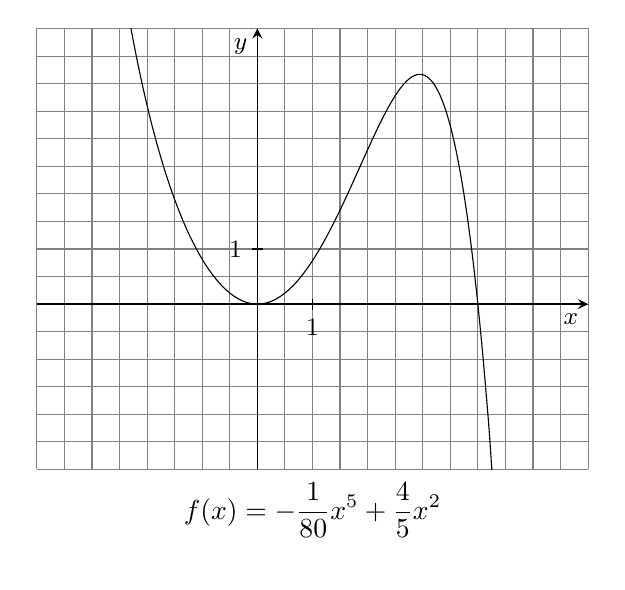
\begin{tikzpicture}[scale=0.7]
  % grid
  \draw[draw=black!50!white] (-4.000, -3.000) grid[step=0.5] (6.000, 5.000);
  % x-axis
  \draw[line width=0.6pt, ->, >=stealth] (-4.000, 0) -- (6.000, 0) node[below left] {\small$x$};
  % x scale
  \draw[line width=0.6pt] (1, 0.1) -- (1, -0.1) node[below] {\small1};
  % y-axis
  \draw[line width=0.6pt, ->, >=stealth] (0, -3.000) -- (0, 5.000) node[below left] {\small$y$};
  % y scale
  \draw[line width=0.6pt] (0.1, 1) -- (-0.1, 1) node[left] {\small1};
  % function
  \begin{scope}
    \clip (-4.000, -3.000) rectangle (6.000, 5.000);
    \draw plot[smooth] coordinates
    {
      ( -4.000,   6.000) ( -3.900,   6.000) ( -3.800,   6.000)
      ( -3.700,   6.000) ( -3.600,   6.000) ( -3.500,   6.000)
      ( -3.400,   6.000) ( -3.300,   6.000) ( -3.200,   6.000)
      ( -3.100,   6.000) ( -3.000,   6.000) ( -2.900,   6.000)
      ( -2.800,   6.000) ( -2.700,   6.000) ( -2.600,   6.000)
      ( -2.500,   6.000) ( -2.400,   5.603) ( -2.300,   5.037)
      ( -2.200,   4.516) ( -2.100,   4.039) ( -2.000,   3.600)
      ( -1.900,   3.198) ( -1.800,   2.828) ( -1.700,   2.489)
      ( -1.600,   2.179) ( -1.500,   1.895) ( -1.400,   1.635)
      ( -1.300,   1.398) ( -1.200,   1.183) ( -1.100,   0.988)
      ( -1.000,   0.812) ( -0.900,   0.655) ( -0.800,   0.516)
      ( -0.700,   0.394) ( -0.600,   0.289) ( -0.500,   0.200)
      ( -0.400,   0.128) ( -0.300,   0.072) ( -0.200,   0.032)
      ( -0.100,   0.008) (  0.000,   0.000) (  0.100,   0.008)
      (  0.200,   0.032) (  0.300,   0.072) (  0.400,   0.128)
      (  0.500,   0.200) (  0.600,   0.287) (  0.700,   0.390)
      (  0.800,   0.508) (  0.900,   0.641) (  1.000,   0.788)
      (  1.100,   0.948) (  1.200,   1.121) (  1.300,   1.306)
      (  1.400,   1.501) (  1.500,   1.705) (  1.600,   1.917)
      (  1.700,   2.135) (  1.800,   2.356) (  1.900,   2.578)
      (  2.000,   2.800) (  2.100,   3.017) (  2.200,   3.228)
      (  2.300,   3.427) (  2.400,   3.613) (  2.500,   3.779)
      (  2.600,   3.923) (  2.700,   4.038) (  2.800,   4.121)
      (  2.900,   4.164) (  3.000,   4.162) (  3.100,   4.109)
      (  3.200,   3.998) (  3.300,   3.820) (  3.400,   3.569)
      (  3.500,   3.235) (  3.600,   2.810) (  3.700,   2.284)
      (  3.800,   1.648) (  3.900,   0.890) (  4.000,   0.000)
      (  4.100,  -1.034) (  4.200,  -2.224) (  4.300,  -3.584)
      (  4.400,  -4.000) (  4.500,  -4.000) (  4.600,  -4.000)
      (  4.700,  -4.000) (  4.800,  -4.000) (  4.900,  -4.000)
      (  5.000,  -4.000) (  5.100,  -4.000) (  5.200,  -4.000)
      (  5.300,  -4.000) (  5.400,  -4.000) (  5.500,  -4.000)
      (  5.600,  -4.000) (  5.700,  -4.000) (  5.800,  -4.000)
      (  5.900,  -4.000) (  6.000,  -4.000)
    };
  \end{scope}
  \node[below] at (1.000, -3.000)
  {%
    \rule[-1.1\baselineskip]{0pt}{2.2\baselineskip}%
    \begin{minipage}{7.000cm}%
      \begin{equation*}%
        f(x)=-\frac{1}{80}x^5+\frac{4}{5}x^2
      \end{equation*}%
    \end{minipage}%
  };
\end{tikzpicture}


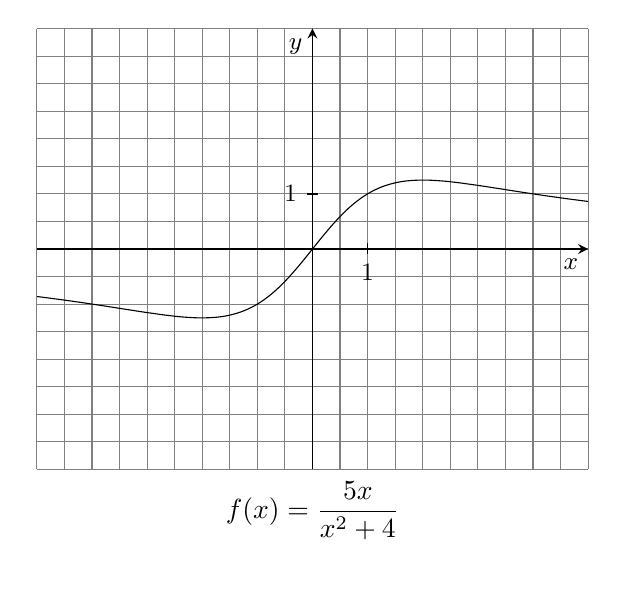
\begin{tikzpicture}[scale=0.7]
  % grid
  \draw[draw=black!50!white] (-5.000, -4.000) grid[step=0.5] (5.000, 4.000);
  % x-axis
  \draw[line width=0.6pt, ->, >=stealth] (-5.000, 0) -- (5.000, 0) node[below left] {\small$x$};
  % x scale
  \draw[line width=0.6pt] (1, 0.1) -- (1, -0.1) node[below] {\small1};
  % y-axis
  \draw[line width=0.6pt, ->, >=stealth] (0, -4.000) -- (0, 4.000) node[below left] {\small$y$};
  % y scale
  \draw[line width=0.6pt] (0.1, 1) -- (-0.1, 1) node[left] {\small1};
  % function
  \begin{scope}
    \clip (-5.000, -4.000) rectangle (5.000, 4.000);
    \draw plot[smooth] coordinates
    {
      ( -5.000,  -0.862) ( -4.900,  -0.875) ( -4.800,  -0.888)
      ( -4.700,  -0.901) ( -4.600,  -0.914) ( -4.500,  -0.928)
      ( -4.400,  -0.942) ( -4.300,  -0.956) ( -4.200,  -0.970)
      ( -4.100,  -0.985) ( -4.000,  -1.000) ( -3.900,  -1.015)
      ( -3.800,  -1.030) ( -3.700,  -1.046) ( -3.600,  -1.061)
      ( -3.500,  -1.077) ( -3.400,  -1.093) ( -3.300,  -1.108)
      ( -3.200,  -1.124) ( -3.100,  -1.139) ( -3.000,  -1.154)
      ( -2.900,  -1.168) ( -2.800,  -1.182) ( -2.700,  -1.196)
      ( -2.600,  -1.208) ( -2.500,  -1.220) ( -2.400,  -1.230)
      ( -2.300,  -1.238) ( -2.200,  -1.244) ( -2.100,  -1.249)
      ( -2.000,  -1.250) ( -1.900,  -1.248) ( -1.800,  -1.243)
      ( -1.700,  -1.234) ( -1.600,  -1.220) ( -1.500,  -1.200)
      ( -1.400,  -1.174) ( -1.300,  -1.142) ( -1.200,  -1.103)
      ( -1.100,  -1.056) ( -1.000,  -1.000) ( -0.900,  -0.936)
      ( -0.800,  -0.862) ( -0.700,  -0.780) ( -0.600,  -0.688)
      ( -0.500,  -0.588) ( -0.400,  -0.481) ( -0.300,  -0.367)
      ( -0.200,  -0.248) ( -0.100,  -0.125) (  0.000,   0.000)
      (  0.100,   0.125) (  0.200,   0.248) (  0.300,   0.367)
      (  0.400,   0.481) (  0.500,   0.588) (  0.600,   0.688)
      (  0.700,   0.780) (  0.800,   0.862) (  0.900,   0.936)
      (  1.000,   1.000) (  1.100,   1.056) (  1.200,   1.103)
      (  1.300,   1.142) (  1.400,   1.174) (  1.500,   1.200)
      (  1.600,   1.220) (  1.700,   1.234) (  1.800,   1.243)
      (  1.900,   1.248) (  2.000,   1.250) (  2.100,   1.249)
      (  2.200,   1.244) (  2.300,   1.238) (  2.400,   1.230)
      (  2.500,   1.220) (  2.600,   1.208) (  2.700,   1.196)
      (  2.800,   1.182) (  2.900,   1.168) (  3.000,   1.154)
      (  3.100,   1.139) (  3.200,   1.124) (  3.300,   1.108)
      (  3.400,   1.093) (  3.500,   1.077) (  3.600,   1.061)
      (  3.700,   1.046) (  3.800,   1.030) (  3.900,   1.015)
      (  4.000,   1.000) (  4.100,   0.985) (  4.200,   0.970)
      (  4.300,   0.956) (  4.400,   0.942) (  4.500,   0.928)
      (  4.600,   0.914) (  4.700,   0.901) (  4.800,   0.888)
      (  4.900,   0.875) (  5.000,   0.862)
    };
  \end{scope}
  \node[below] at (0.000, -4.000)
  {%
    \rule[-1.1\baselineskip]{0pt}{2.2\baselineskip}%
    \begin{minipage}{7.000cm}%
      \begin{equation*}%
        f(x)=\frac{5x}{x^2+4}
      \end{equation*}%
    \end{minipage}%
  };
\end{tikzpicture}

\hfill
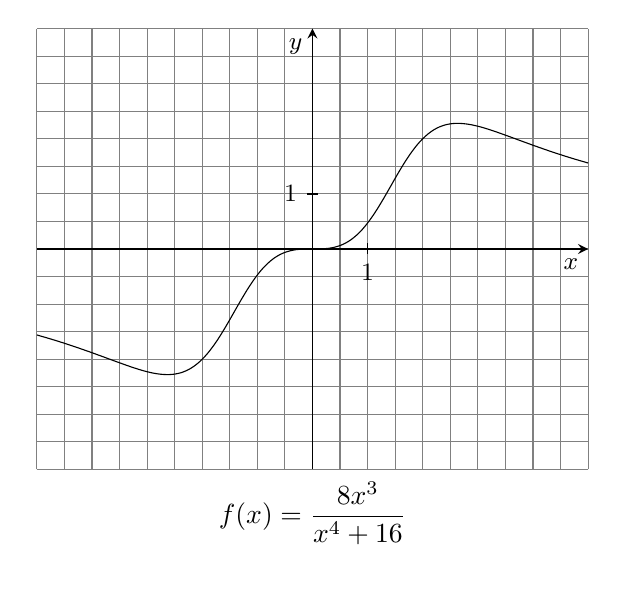
\begin{tikzpicture}[scale=0.7]
  % grid
  \draw[draw=black!50!white] (-5.000, -4.000) grid[step=0.5] (5.000, 4.000);
  % x-axis
  \draw[line width=0.6pt, ->, >=stealth] (-5.000, 0) -- (5.000, 0) node[below left] {\small$x$};
  % x scale
  \draw[line width=0.6pt] (1, 0.1) -- (1, -0.1) node[below] {\small1};
  % y-axis
  \draw[line width=0.6pt, ->, >=stealth] (0, -4.000) -- (0, 4.000) node[below left] {\small$y$};
  % y scale
  \draw[line width=0.6pt] (0.1, 1) -- (-0.1, 1) node[left] {\small1};
  % function
  \begin{scope}
    \clip (-5.000, -4.000) rectangle (5.000, 4.000);
    \draw plot[smooth] coordinates
    {
      ( -5.000,  -1.560) ( -4.900,  -1.589) ( -4.800,  -1.618)
      ( -4.700,  -1.648) ( -4.600,  -1.679) ( -4.500,  -1.711)
      ( -4.400,  -1.744) ( -4.300,  -1.777) ( -4.200,  -1.812)
      ( -4.100,  -1.847) ( -4.000,  -1.882) ( -3.900,  -1.919)
      ( -3.800,  -1.955) ( -3.700,  -1.992) ( -3.600,  -2.029)
      ( -3.500,  -2.065) ( -3.400,  -2.101) ( -3.300,  -2.136)
      ( -3.200,  -2.169) ( -3.100,  -2.200) ( -3.000,  -2.227)
      ( -2.900,  -2.250) ( -2.800,  -2.267) ( -2.700,  -2.277)
      ( -2.600,  -2.279) ( -2.500,  -2.270) ( -2.400,  -2.249)
      ( -2.300,  -2.213) ( -2.200,  -2.161) ( -2.100,  -2.090)
      ( -2.000,  -2.000) ( -1.900,  -1.890) ( -1.800,  -1.761)
      ( -1.700,  -1.614) ( -1.600,  -1.453) ( -1.500,  -1.282)
      ( -1.400,  -1.106) ( -1.300,  -0.932) ( -1.200,  -0.765)
      ( -1.100,  -0.610) ( -1.000,  -0.471) ( -0.900,  -0.350)
      ( -0.800,  -0.250) ( -0.700,  -0.169) ( -0.600,  -0.107)
      ( -0.500,  -0.062) ( -0.400,  -0.032) ( -0.300,  -0.013)
      ( -0.200,  -0.004) ( -0.100,  -0.000) (  0.000,   0.000)
      (  0.100,   0.000) (  0.200,   0.004) (  0.300,   0.013)
      (  0.400,   0.032) (  0.500,   0.062) (  0.600,   0.107)
      (  0.700,   0.169) (  0.800,   0.250) (  0.900,   0.350)
      (  1.000,   0.471) (  1.100,   0.610) (  1.200,   0.765)
      (  1.300,   0.932) (  1.400,   1.106) (  1.500,   1.282)
      (  1.600,   1.453) (  1.700,   1.614) (  1.800,   1.761)
      (  1.900,   1.890) (  2.000,   2.000) (  2.100,   2.090)
      (  2.200,   2.161) (  2.300,   2.213) (  2.400,   2.249)
      (  2.500,   2.270) (  2.600,   2.279) (  2.700,   2.277)
      (  2.800,   2.267) (  2.900,   2.250) (  3.000,   2.227)
      (  3.100,   2.200) (  3.200,   2.169) (  3.300,   2.136)
      (  3.400,   2.101) (  3.500,   2.065) (  3.600,   2.029)
      (  3.700,   1.992) (  3.800,   1.955) (  3.900,   1.919)
      (  4.000,   1.882) (  4.100,   1.847) (  4.200,   1.812)
      (  4.300,   1.777) (  4.400,   1.744) (  4.500,   1.711)
      (  4.600,   1.679) (  4.700,   1.648) (  4.800,   1.618)
      (  4.900,   1.589) (  5.000,   1.560)
    };
  \end{scope}
  \node[below] at (0.000, -4.000)
  {%
    \rule[-1.1\baselineskip]{0pt}{2.2\baselineskip}%
    \begin{minipage}{7.000cm}%
      \begin{equation*}%
        f(x)=\frac{8x^3}{x^4+16}
      \end{equation*}%
    \end{minipage}%
  };
\end{tikzpicture}


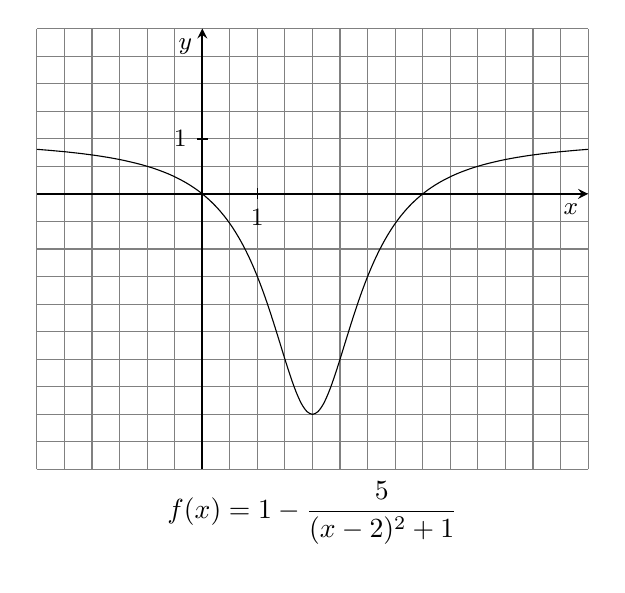
\begin{tikzpicture}[scale=0.7]
  % grid
  \draw[draw=black!50!white] (-3.000, -5.000) grid[step=0.5] (7.000, 3.000);
  % x-axis
  \draw[line width=0.6pt, ->, >=stealth] (-3.000, 0) -- (7.000, 0) node[below left] {\small$x$};
  % x scale
  \draw[line width=0.6pt] (1, 0.1) -- (1, -0.1) node[below] {\small1};
  % y-axis
  \draw[line width=0.6pt, ->, >=stealth] (0, -5.000) -- (0, 3.000) node[below left] {\small$y$};
  % y scale
  \draw[line width=0.6pt] (0.1, 1) -- (-0.1, 1) node[left] {\small1};
  % function
  \begin{scope}
    \clip (-3.000, -5.000) rectangle (7.000, 3.000);
    \draw plot[smooth] coordinates
    {
      ( -3.000,   0.808) ( -2.900,   0.800) ( -2.800,   0.792)
      ( -2.700,   0.783) ( -2.600,   0.774) ( -2.500,   0.765)
      ( -2.400,   0.754) ( -2.300,   0.743) ( -2.200,   0.732)
      ( -2.100,   0.719) ( -2.000,   0.706) ( -1.900,   0.692)
      ( -1.800,   0.676) ( -1.700,   0.660) ( -1.600,   0.642)
      ( -1.500,   0.623) ( -1.400,   0.602) ( -1.300,   0.579)
      ( -1.200,   0.555) ( -1.100,   0.529) ( -1.000,   0.500)
      ( -0.900,   0.469) ( -0.800,   0.434) ( -0.700,   0.397)
      ( -0.600,   0.356) ( -0.500,   0.310) ( -0.400,   0.260)
      ( -0.300,   0.205) ( -0.200,   0.144) ( -0.100,   0.076)
      (  0.000,   0.000) (  0.100,  -0.085) (  0.200,  -0.179)
      (  0.300,  -0.285) (  0.400,  -0.404) (  0.500,  -0.538)
      (  0.600,  -0.689) (  0.700,  -0.859) (  0.800,  -1.049)
      (  0.900,  -1.262) (  1.000,  -1.500) (  1.100,  -1.762)
      (  1.200,  -2.049) (  1.300,  -2.356) (  1.400,  -2.676)
      (  1.500,  -3.000) (  1.600,  -3.310) (  1.700,  -3.587)
      (  1.800,  -3.808) (  1.900,  -3.950) (  2.000,  -4.000)
      (  2.100,  -3.950) (  2.200,  -3.808) (  2.300,  -3.587)
      (  2.400,  -3.310) (  2.500,  -3.000) (  2.600,  -2.676)
      (  2.700,  -2.356) (  2.800,  -2.049) (  2.900,  -1.762)
      (  3.000,  -1.500) (  3.100,  -1.262) (  3.200,  -1.049)
      (  3.300,  -0.859) (  3.400,  -0.689) (  3.500,  -0.538)
      (  3.600,  -0.404) (  3.700,  -0.285) (  3.800,  -0.179)
      (  3.900,  -0.085) (  4.000,   0.000) (  4.100,   0.076)
      (  4.200,   0.144) (  4.300,   0.205) (  4.400,   0.260)
      (  4.500,   0.310) (  4.600,   0.356) (  4.700,   0.397)
      (  4.800,   0.434) (  4.900,   0.469) (  5.000,   0.500)
      (  5.100,   0.529) (  5.200,   0.555) (  5.300,   0.579)
      (  5.400,   0.602) (  5.500,   0.623) (  5.600,   0.642)
      (  5.700,   0.660) (  5.800,   0.676) (  5.900,   0.692)
      (  6.000,   0.706) (  6.100,   0.719) (  6.200,   0.732)
      (  6.300,   0.743) (  6.400,   0.754) (  6.500,   0.765)
      (  6.600,   0.774) (  6.700,   0.783) (  6.800,   0.792)
      (  6.900,   0.800) (  7.000,   0.808)
    };
  \end{scope}
  \node[below] at (2.000, -5.000)
  {%
    \rule[-1.1\baselineskip]{0pt}{2.2\baselineskip}%
    \begin{minipage}{7.000cm}%
      \begin{equation*}%
        f(x)=1-\frac{5}{(x-2)^2+1}
      \end{equation*}%
    \end{minipage}%
  };
\end{tikzpicture}

\hfill
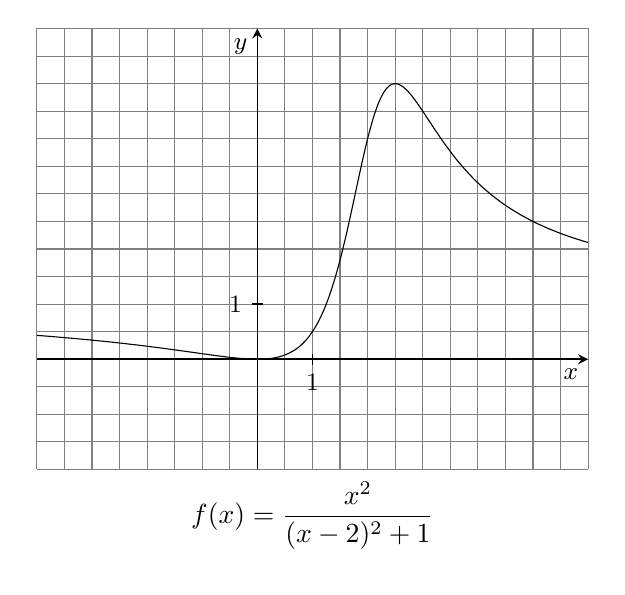
\begin{tikzpicture}[scale=0.7]
  % grid
  \draw[draw=black!50!white] (-4.000, -2.000) grid[step=0.5] (6.000, 6.000);
  % x-axis
  \draw[line width=0.6pt, ->, >=stealth] (-4.000, 0) -- (6.000, 0) node[below left] {\small$x$};
  % x scale
  \draw[line width=0.6pt] (1, 0.1) -- (1, -0.1) node[below] {\small1};
  % y-axis
  \draw[line width=0.6pt, ->, >=stealth] (0, -2.000) -- (0, 6.000) node[below left] {\small$y$};
  % y scale
  \draw[line width=0.6pt] (0.1, 1) -- (-0.1, 1) node[left] {\small1};
  % function
  \begin{scope}
    \clip (-4.000, -2.000) rectangle (6.000, 6.000);
    \draw plot[smooth] coordinates
    {
      ( -4.000,   0.432) ( -3.900,   0.425) ( -3.800,   0.417)
      ( -3.700,   0.409) ( -3.600,   0.400) ( -3.500,   0.392)
      ( -3.400,   0.383) ( -3.300,   0.374) ( -3.200,   0.365)
      ( -3.100,   0.356) ( -3.000,   0.346) ( -2.900,   0.336)
      ( -2.800,   0.326) ( -2.700,   0.316) ( -2.600,   0.305)
      ( -2.500,   0.294) ( -2.400,   0.283) ( -2.300,   0.271)
      ( -2.200,   0.260) ( -2.100,   0.248) ( -2.000,   0.235)
      ( -1.900,   0.223) ( -1.800,   0.210) ( -1.700,   0.197)
      ( -1.600,   0.183) ( -1.500,   0.170) ( -1.400,   0.156)
      ( -1.300,   0.142) ( -1.200,   0.128) ( -1.100,   0.114)
      ( -1.000,   0.100) ( -0.900,   0.086) ( -0.800,   0.072)
      ( -0.700,   0.059) ( -0.600,   0.046) ( -0.500,   0.034)
      ( -0.400,   0.024) ( -0.300,   0.014) ( -0.200,   0.007)
      ( -0.100,   0.002) (  0.000,   0.000) (  0.100,   0.002)
      (  0.200,   0.009) (  0.300,   0.023) (  0.400,   0.045)
      (  0.500,   0.077) (  0.600,   0.122) (  0.700,   0.182)
      (  0.800,   0.262) (  0.900,   0.367) (  1.000,   0.500)
      (  1.100,   0.669) (  1.200,   0.878) (  1.300,   1.134)
      (  1.400,   1.441) (  1.500,   1.800) (  1.600,   2.207)
      (  1.700,   2.651) (  1.800,   3.115) (  1.900,   3.574)
      (  2.000,   4.000) (  2.100,   4.366) (  2.200,   4.654)
      (  2.300,   4.853) (  2.400,   4.966) (  2.500,   5.000)
      (  2.600,   4.971) (  2.700,   4.893) (  2.800,   4.780)
      (  2.900,   4.646) (  3.000,   4.500) (  3.100,   4.348)
      (  3.200,   4.197) (  3.300,   4.048) (  3.400,   3.905)
      (  3.500,   3.769) (  3.600,   3.640) (  3.700,   3.519)
      (  3.800,   3.406) (  3.900,   3.299) (  4.000,   3.200)
      (  4.100,   3.107) (  4.200,   3.021) (  4.300,   2.940)
      (  4.400,   2.864) (  4.500,   2.793) (  4.600,   2.727)
      (  4.700,   2.665) (  4.800,   2.606) (  4.900,   2.552)
      (  5.000,   2.500) (  5.100,   2.451) (  5.200,   2.406)
      (  5.300,   2.362) (  5.400,   2.322) (  5.500,   2.283)
      (  5.600,   2.246) (  5.700,   2.212) (  5.800,   2.179)
      (  5.900,   2.147) (  6.000,   2.118)
    };
  \end{scope}
  \node[below] at (1.000, -2.000)
  {%
    \rule[-1.1\baselineskip]{0pt}{2.2\baselineskip}%
    \begin{minipage}{7.000cm}%
      \begin{equation*}%
        f(x)=\frac{x^2}{(x-2)^2+1}
      \end{equation*}%
    \end{minipage}%
  };
\end{tikzpicture}


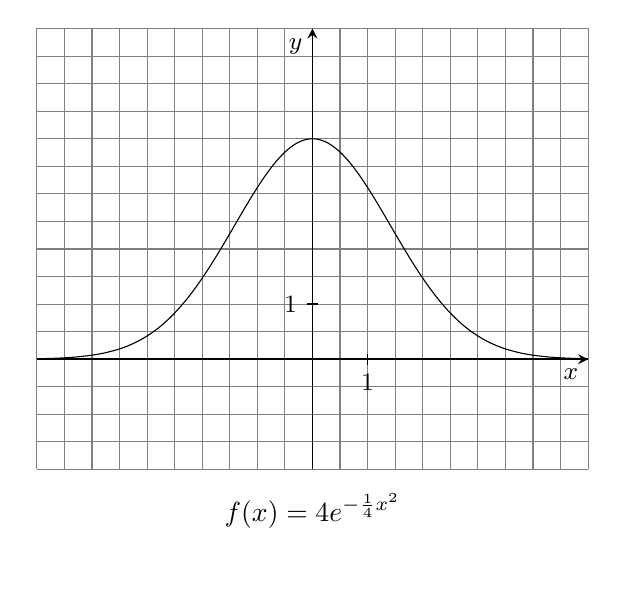
\begin{tikzpicture}[scale=0.7]
  % grid
  \draw[draw=black!50!white] (-5.000, -2.000) grid[step=0.5] (5.000, 6.000);
  % x-axis
  \draw[line width=0.6pt, ->, >=stealth] (-5.000, 0) -- (5.000, 0) node[below left] {\small$x$};
  % x scale
  \draw[line width=0.6pt] (1, 0.1) -- (1, -0.1) node[below] {\small1};
  % y-axis
  \draw[line width=0.6pt, ->, >=stealth] (0, -2.000) -- (0, 6.000) node[below left] {\small$y$};
  % y scale
  \draw[line width=0.6pt] (0.1, 1) -- (-0.1, 1) node[left] {\small1};
  % function
  \begin{scope}
    \clip (-5.000, -2.000) rectangle (5.000, 6.000);
    \draw plot[smooth] coordinates
    {
      ( -5.000,   0.008) ( -4.900,   0.010) ( -4.800,   0.013)
      ( -4.700,   0.016) ( -4.600,   0.020) ( -4.500,   0.025)
      ( -4.400,   0.032) ( -4.300,   0.039) ( -4.200,   0.049)
      ( -4.100,   0.060) ( -4.000,   0.073) ( -3.900,   0.089)
      ( -3.800,   0.108) ( -3.700,   0.131) ( -3.600,   0.157)
      ( -3.500,   0.187) ( -3.400,   0.222) ( -3.300,   0.263)
      ( -3.200,   0.309) ( -3.100,   0.362) ( -3.000,   0.422)
      ( -2.900,   0.489) ( -2.800,   0.563) ( -2.700,   0.646)
      ( -2.600,   0.738) ( -2.500,   0.838) ( -2.400,   0.948)
      ( -2.300,   1.066) ( -2.200,   1.193) ( -2.100,   1.328)
      ( -2.000,   1.472) ( -1.900,   1.622) ( -1.800,   1.779)
      ( -1.700,   1.942) ( -1.600,   2.109) ( -1.500,   2.279)
      ( -1.400,   2.451) ( -1.300,   2.622) ( -1.200,   2.791)
      ( -1.100,   2.956) ( -1.000,   3.115) ( -0.900,   3.267)
      ( -0.800,   3.409) ( -0.700,   3.539) ( -0.600,   3.656)
      ( -0.500,   3.758) ( -0.400,   3.843) ( -0.300,   3.911)
      ( -0.200,   3.960) ( -0.100,   3.990) (  0.000,   4.000)
      (  0.100,   3.990) (  0.200,   3.960) (  0.300,   3.911)
      (  0.400,   3.843) (  0.500,   3.758) (  0.600,   3.656)
      (  0.700,   3.539) (  0.800,   3.409) (  0.900,   3.267)
      (  1.000,   3.115) (  1.100,   2.956) (  1.200,   2.791)
      (  1.300,   2.622) (  1.400,   2.451) (  1.500,   2.279)
      (  1.600,   2.109) (  1.700,   1.942) (  1.800,   1.779)
      (  1.900,   1.622) (  2.000,   1.472) (  2.100,   1.328)
      (  2.200,   1.193) (  2.300,   1.066) (  2.400,   0.948)
      (  2.500,   0.838) (  2.600,   0.738) (  2.700,   0.646)
      (  2.800,   0.563) (  2.900,   0.489) (  3.000,   0.422)
      (  3.100,   0.362) (  3.200,   0.309) (  3.300,   0.263)
      (  3.400,   0.222) (  3.500,   0.187) (  3.600,   0.157)
      (  3.700,   0.131) (  3.800,   0.108) (  3.900,   0.089)
      (  4.000,   0.073) (  4.100,   0.060) (  4.200,   0.049)
      (  4.300,   0.039) (  4.400,   0.032) (  4.500,   0.025)
      (  4.600,   0.020) (  4.700,   0.016) (  4.800,   0.013)
      (  4.900,   0.010) (  5.000,   0.008)
    };
  \end{scope}
  \node[below] at (0.000, -2.000)
  {%
    \rule[-1.1\baselineskip]{0pt}{2.2\baselineskip}%
    \begin{minipage}{7.000cm}%
      \begin{equation*}%
        f(x)=4e^{-\frac{1}{4}x^2}
      \end{equation*}%
    \end{minipage}%
  };
\end{tikzpicture}

\hfill
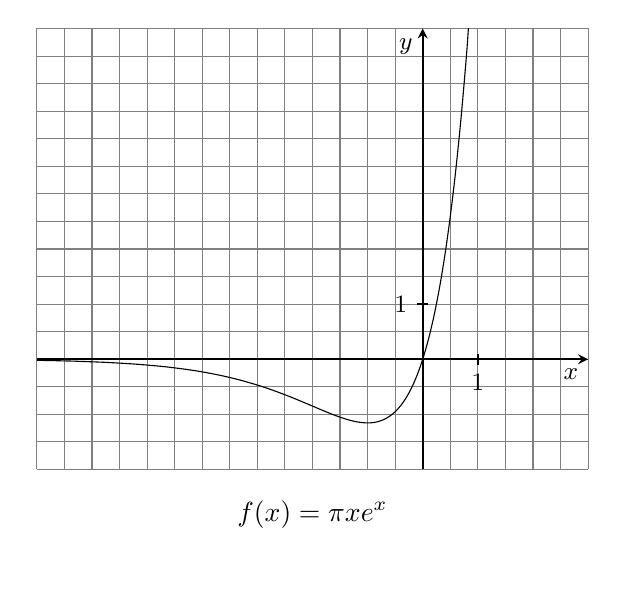
\begin{tikzpicture}[scale=0.7]
  % grid
  \draw[draw=black!50!white] (-7.000, -2.000) grid[step=0.5] (3.000, 6.000);
  % x-axis
  \draw[line width=0.6pt, ->, >=stealth] (-7.000, 0) -- (3.000, 0) node[below left] {\small$x$};
  % x scale
  \draw[line width=0.6pt] (1, 0.1) -- (1, -0.1) node[below] {\small1};
  % y-axis
  \draw[line width=0.6pt, ->, >=stealth] (0, -2.000) -- (0, 6.000) node[below left] {\small$y$};
  % y scale
  \draw[line width=0.6pt] (0.1, 1) -- (-0.1, 1) node[left] {\small1};
  % function
  \begin{scope}
    \clip (-7.000, -2.000) rectangle (3.000, 6.000);
    \draw plot[smooth] coordinates
    {
      ( -7.000,  -0.020) ( -6.900,  -0.022) ( -6.800,  -0.024)
      ( -6.700,  -0.026) ( -6.600,  -0.028) ( -6.500,  -0.031)
      ( -6.400,  -0.033) ( -6.300,  -0.036) ( -6.200,  -0.040)
      ( -6.100,  -0.043) ( -6.000,  -0.047) ( -5.900,  -0.051)
      ( -5.800,  -0.055) ( -5.700,  -0.060) ( -5.600,  -0.065)
      ( -5.500,  -0.071) ( -5.400,  -0.077) ( -5.300,  -0.083)
      ( -5.200,  -0.090) ( -5.100,  -0.098) ( -5.000,  -0.106)
      ( -4.900,  -0.115) ( -4.800,  -0.124) ( -4.700,  -0.134)
      ( -4.600,  -0.145) ( -4.500,  -0.157) ( -4.400,  -0.170)
      ( -4.300,  -0.183) ( -4.200,  -0.198) ( -4.100,  -0.213)
      ( -4.000,  -0.230) ( -3.900,  -0.248) ( -3.800,  -0.267)
      ( -3.700,  -0.287) ( -3.600,  -0.309) ( -3.500,  -0.332)
      ( -3.400,  -0.356) ( -3.300,  -0.382) ( -3.200,  -0.410)
      ( -3.100,  -0.439) ( -3.000,  -0.469) ( -2.900,  -0.501)
      ( -2.800,  -0.535) ( -2.700,  -0.570) ( -2.600,  -0.607)
      ( -2.500,  -0.645) ( -2.400,  -0.684) ( -2.300,  -0.724)
      ( -2.200,  -0.766) ( -2.100,  -0.808) ( -2.000,  -0.850)
      ( -1.900,  -0.893) ( -1.800,  -0.935) ( -1.700,  -0.976)
      ( -1.600,  -1.015) ( -1.500,  -1.051) ( -1.400,  -1.085)
      ( -1.300,  -1.113) ( -1.200,  -1.135) ( -1.100,  -1.150)
      ( -1.000,  -1.156) ( -0.900,  -1.150) ( -0.800,  -1.129)
      ( -0.700,  -1.092) ( -0.600,  -1.034) ( -0.500,  -0.953)
      ( -0.400,  -0.842) ( -0.300,  -0.698) ( -0.200,  -0.514)
      ( -0.100,  -0.284) (  0.000,   0.000) (  0.100,   0.347)
      (  0.200,   0.767) (  0.300,   1.272) (  0.400,   1.875)
      (  0.500,   2.590) (  0.600,   3.435) (  0.700,   4.428)
      (  0.800,   5.593) (  0.900,   6.954) (  1.000,   7.000)
      (  1.100,   7.000) (  1.200,   7.000) (  1.300,   7.000)
      (  1.400,   7.000) (  1.500,   7.000) (  1.600,   7.000)
      (  1.700,   7.000) (  1.800,   7.000) (  1.900,   7.000)
      (  2.000,   7.000) (  2.100,   7.000) (  2.200,   7.000)
      (  2.300,   7.000) (  2.400,   7.000) (  2.500,   7.000)
      (  2.600,   7.000) (  2.700,   7.000) (  2.800,   7.000)
      (  2.900,   7.000) (  3.000,   7.000)
    };
  \end{scope}
  \node[below] at (-2.000, -2.000)
  {%
    \rule[-1.1\baselineskip]{0pt}{2.2\baselineskip}%
    \begin{minipage}{7.000cm}%
      \begin{equation*}%
        f(x)=\pi xe^x
      \end{equation*}%
    \end{minipage}%
  };
\end{tikzpicture}


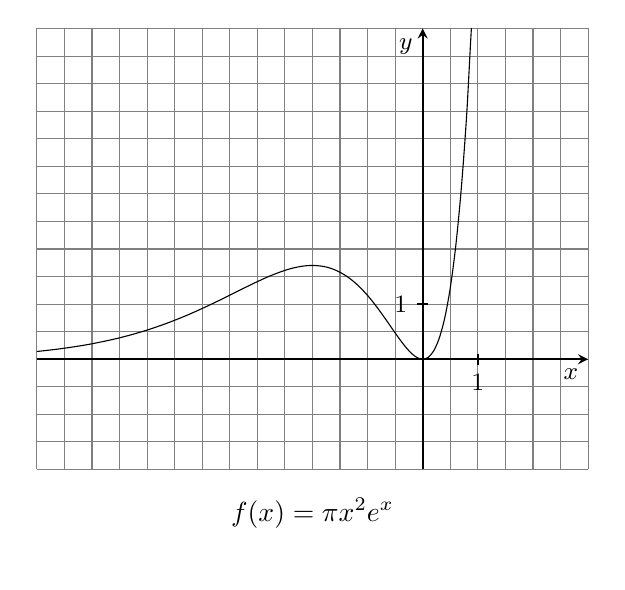
\begin{tikzpicture}[scale=0.7]
  % grid
  \draw[draw=black!50!white] (-7.000, -2.000) grid[step=0.5] (3.000, 6.000);
  % x-axis
  \draw[line width=0.6pt, ->, >=stealth] (-7.000, 0) -- (3.000, 0) node[below left] {\small$x$};
  % x scale
  \draw[line width=0.6pt] (1, 0.1) -- (1, -0.1) node[below] {\small1};
  % y-axis
  \draw[line width=0.6pt, ->, >=stealth] (0, -2.000) -- (0, 6.000) node[below left] {\small$y$};
  % y scale
  \draw[line width=0.6pt] (0.1, 1) -- (-0.1, 1) node[left] {\small1};
  % function
  \begin{scope}
    \clip (-7.000, -2.000) rectangle (3.000, 6.000);
    \draw plot[smooth] coordinates
    {
      ( -7.000,   0.140) ( -6.900,   0.151) ( -6.800,   0.162)
      ( -6.700,   0.174) ( -6.600,   0.186) ( -6.500,   0.200)
      ( -6.400,   0.214) ( -6.300,   0.229) ( -6.200,   0.245)
      ( -6.100,   0.262) ( -6.000,   0.280) ( -5.900,   0.300)
      ( -5.800,   0.320) ( -5.700,   0.342) ( -5.600,   0.364)
      ( -5.500,   0.388) ( -5.400,   0.414) ( -5.300,   0.440)
      ( -5.200,   0.469) ( -5.100,   0.498) ( -5.000,   0.529)
      ( -4.900,   0.562) ( -4.800,   0.596) ( -4.700,   0.631)
      ( -4.600,   0.668) ( -4.500,   0.707) ( -4.400,   0.747)
      ( -4.300,   0.788) ( -4.200,   0.831) ( -4.100,   0.875)
      ( -4.000,   0.921) ( -3.900,   0.967) ( -3.800,   1.015)
      ( -3.700,   1.063) ( -3.600,   1.112) ( -3.500,   1.162)
      ( -3.400,   1.212) ( -3.300,   1.262) ( -3.200,   1.311)
      ( -3.100,   1.360) ( -3.000,   1.408) ( -2.900,   1.454)
      ( -2.800,   1.498) ( -2.700,   1.539) ( -2.600,   1.577)
      ( -2.500,   1.612) ( -2.400,   1.642) ( -2.300,   1.666)
      ( -2.200,   1.685) ( -2.100,   1.697) ( -2.000,   1.701)
      ( -1.900,   1.696) ( -1.800,   1.683) ( -1.700,   1.659)
      ( -1.600,   1.624) ( -1.500,   1.577) ( -1.400,   1.518)
      ( -1.300,   1.447) ( -1.200,   1.363) ( -1.100,   1.265)
      ( -1.000,   1.156) ( -0.900,   1.035) ( -0.800,   0.903)
      ( -0.700,   0.764) ( -0.600,   0.621) ( -0.500,   0.476)
      ( -0.400,   0.337) ( -0.300,   0.209) ( -0.200,   0.103)
      ( -0.100,   0.028) (  0.000,   0.000) (  0.100,   0.035)
      (  0.200,   0.153) (  0.300,   0.382) (  0.400,   0.750)
      (  0.500,   1.295) (  0.600,   2.061) (  0.700,   3.100)
      (  0.800,   4.475) (  0.900,   6.259) (  1.000,   7.000)
      (  1.100,   7.000) (  1.200,   7.000) (  1.300,   7.000)
      (  1.400,   7.000) (  1.500,   7.000) (  1.600,   7.000)
      (  1.700,   7.000) (  1.800,   7.000) (  1.900,   7.000)
      (  2.000,   7.000) (  2.100,   7.000) (  2.200,   7.000)
      (  2.300,   7.000) (  2.400,   7.000) (  2.500,   7.000)
      (  2.600,   7.000) (  2.700,   7.000) (  2.800,   7.000)
      (  2.900,   7.000) (  3.000,   7.000)
    };
  \end{scope}
  \node[below] at (-2.000, -2.000)
  {%
    \rule[-1.1\baselineskip]{0pt}{2.2\baselineskip}%
    \begin{minipage}{7.000cm}%
      \begin{equation*}%
        f(x)=\pi x^2e^x
      \end{equation*}%
    \end{minipage}%
  };
\end{tikzpicture}

\hfill
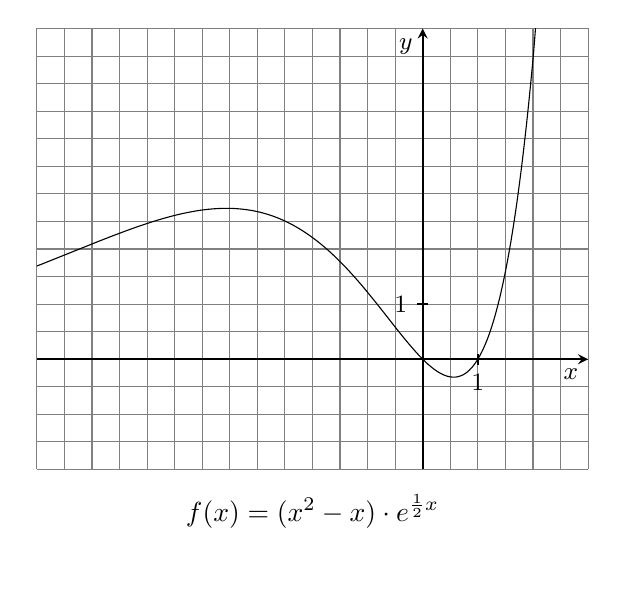
\begin{tikzpicture}[scale=0.7]
  % grid
  \draw[draw=black!50!white] (-7.000, -2.000) grid[step=0.5] (3.000, 6.000);
  % x-axis
  \draw[line width=0.6pt, ->, >=stealth] (-7.000, 0) -- (3.000, 0) node[below left] {\small$x$};
  % x scale
  \draw[line width=0.6pt] (1, 0.1) -- (1, -0.1) node[below] {\small1};
  % y-axis
  \draw[line width=0.6pt, ->, >=stealth] (0, -2.000) -- (0, 6.000) node[below left] {\small$y$};
  % y scale
  \draw[line width=0.6pt] (0.1, 1) -- (-0.1, 1) node[left] {\small1};
  % function
  \begin{scope}
    \clip (-7.000, -2.000) rectangle (3.000, 6.000);
    \draw plot[smooth] coordinates
    {
      ( -7.000,   1.691) ( -6.900,   1.730) ( -6.800,   1.770)
      ( -6.700,   1.810) ( -6.600,   1.850) ( -6.500,   1.890)
      ( -6.400,   1.930) ( -6.300,   1.971) ( -6.200,   2.011)
      ( -6.100,   2.051) ( -6.000,   2.091) ( -5.900,   2.131)
      ( -5.800,   2.170) ( -5.700,   2.209) ( -5.600,   2.248)
      ( -5.500,   2.285) ( -5.400,   2.323) ( -5.300,   2.359)
      ( -5.200,   2.395) ( -5.100,   2.429) ( -5.000,   2.463)
      ( -4.900,   2.495) ( -4.800,   2.526) ( -4.700,   2.555)
      ( -4.600,   2.583) ( -4.500,   2.609) ( -4.400,   2.633)
      ( -4.300,   2.655) ( -4.200,   2.674) ( -4.100,   2.692)
      ( -4.000,   2.707) ( -3.900,   2.719) ( -3.800,   2.728)
      ( -3.700,   2.734) ( -3.600,   2.737) ( -3.500,   2.737)
      ( -3.400,   2.733) ( -3.300,   2.725) ( -3.200,   2.713)
      ( -3.100,   2.698) ( -3.000,   2.678) ( -2.900,   2.653)
      ( -2.800,   2.624) ( -2.700,   2.590) ( -2.600,   2.551)
      ( -2.500,   2.507) ( -2.400,   2.458) ( -2.300,   2.403)
      ( -2.200,   2.343) ( -2.100,   2.278) ( -2.000,   2.207)
      ( -1.900,   2.131) ( -1.800,   2.049) ( -1.700,   1.962)
      ( -1.600,   1.869) ( -1.500,   1.771) ( -1.400,   1.669)
      ( -1.300,   1.561) ( -1.200,   1.449) ( -1.100,   1.333)
      ( -1.000,   1.213) ( -0.900,   1.090) ( -0.800,   0.965)
      ( -0.700,   0.839) ( -0.600,   0.711) ( -0.500,   0.584)
      ( -0.400,   0.458) ( -0.300,   0.336) ( -0.200,   0.217)
      ( -0.100,   0.105) (  0.000,   0.000) (  0.100,  -0.095)
      (  0.200,  -0.177) (  0.300,  -0.244) (  0.400,  -0.293)
      (  0.500,  -0.321) (  0.600,  -0.324) (  0.700,  -0.298)
      (  0.800,  -0.239) (  0.900,  -0.141) (  1.000,   0.000)
      (  1.100,   0.191) (  1.200,   0.437) (  1.300,   0.747)
      (  1.400,   1.128) (  1.500,   1.588) (  1.600,   2.137)
      (  1.700,   2.784) (  1.800,   3.542) (  1.900,   4.422)
      (  2.000,   5.437) (  2.100,   6.601) (  2.200,   7.000)
      (  2.300,   7.000) (  2.400,   7.000) (  2.500,   7.000)
      (  2.600,   7.000) (  2.700,   7.000) (  2.800,   7.000)
      (  2.900,   7.000) (  3.000,   7.000)
    };
  \end{scope}
  \node[below] at (-2.000, -2.000)
  {%
    \rule[-1.1\baselineskip]{0pt}{2.2\baselineskip}%
    \begin{minipage}{7.000cm}%
      \begin{equation*}%
        f(x)=(x^2-x)\cdot e^{\frac{1}{2}x}
      \end{equation*}%
    \end{minipage}%
  };
\end{tikzpicture}


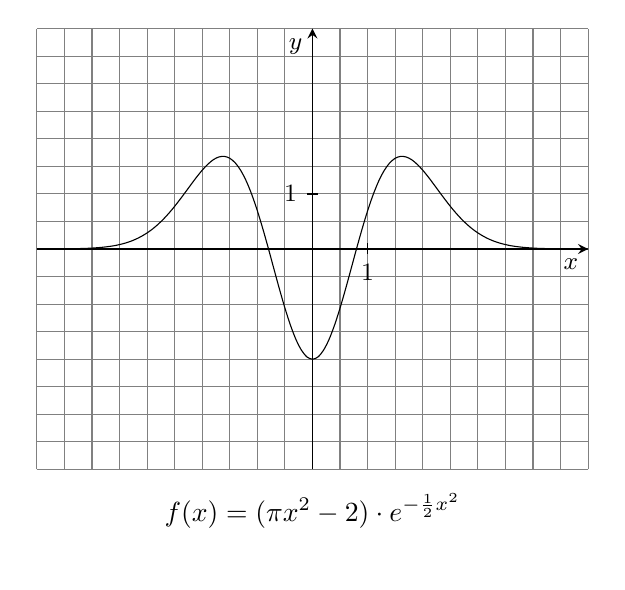
\begin{tikzpicture}[scale=0.7]
  % grid
  \draw[draw=black!50!white] (-5.000, -4.000) grid[step=0.5] (5.000, 4.000);
  % x-axis
  \draw[line width=0.6pt, ->, >=stealth] (-5.000, 0) -- (5.000, 0) node[below left] {\small$x$};
  % x scale
  \draw[line width=0.6pt] (1, 0.1) -- (1, -0.1) node[below] {\small1};
  % y-axis
  \draw[line width=0.6pt, ->, >=stealth] (0, -4.000) -- (0, 4.000) node[below left] {\small$y$};
  % y scale
  \draw[line width=0.6pt] (0.1, 1) -- (-0.1, 1) node[left] {\small1};
  % function
  \begin{scope}
    \clip (-5.000, -4.000) rectangle (5.000, 4.000);
    \draw plot[smooth] coordinates
    {
      ( -5.000,   0.000) ( -4.900,   0.000) ( -4.800,   0.001)
      ( -4.700,   0.001) ( -4.600,   0.002) ( -4.500,   0.002)
      ( -4.400,   0.004) ( -4.300,   0.005) ( -4.200,   0.008)
      ( -4.100,   0.011) ( -4.000,   0.016) ( -3.900,   0.023)
      ( -3.800,   0.032) ( -3.700,   0.044) ( -3.600,   0.059)
      ( -3.500,   0.080) ( -3.400,   0.106) ( -3.300,   0.139)
      ( -3.200,   0.180) ( -3.100,   0.231) ( -3.000,   0.292)
      ( -2.900,   0.364) ( -2.800,   0.449) ( -2.700,   0.546)
      ( -2.600,   0.655) ( -2.500,   0.775) ( -2.400,   0.904)
      ( -2.300,   1.038) ( -2.200,   1.174) ( -2.100,   1.307)
      ( -2.000,   1.430) ( -1.900,   1.536) ( -1.800,   1.619)
      ( -1.700,   1.669) ( -1.600,   1.680) ( -1.500,   1.646)
      ( -1.400,   1.560) ( -1.300,   1.422) ( -1.200,   1.229)
      ( -1.100,   0.984) ( -1.000,   0.692) ( -0.900,   0.363)
      ( -0.800,   0.008) ( -0.700,  -0.361) ( -0.600,  -0.726)
      ( -0.500,  -1.072) ( -0.400,  -1.382) ( -0.300,  -1.642)
      ( -0.200,  -1.837) ( -0.100,  -1.959) (  0.000,  -2.000)
      (  0.100,  -1.959) (  0.200,  -1.837) (  0.300,  -1.642)
      (  0.400,  -1.382) (  0.500,  -1.072) (  0.600,  -0.726)
      (  0.700,  -0.361) (  0.800,   0.008) (  0.900,   0.363)
      (  1.000,   0.692) (  1.100,   0.984) (  1.200,   1.229)
      (  1.300,   1.422) (  1.400,   1.560) (  1.500,   1.646)
      (  1.600,   1.680) (  1.700,   1.669) (  1.800,   1.619)
      (  1.900,   1.536) (  2.000,   1.430) (  2.100,   1.307)
      (  2.200,   1.174) (  2.300,   1.038) (  2.400,   0.904)
      (  2.500,   0.775) (  2.600,   0.655) (  2.700,   0.546)
      (  2.800,   0.449) (  2.900,   0.364) (  3.000,   0.292)
      (  3.100,   0.231) (  3.200,   0.180) (  3.300,   0.139)
      (  3.400,   0.106) (  3.500,   0.080) (  3.600,   0.059)
      (  3.700,   0.044) (  3.800,   0.032) (  3.900,   0.023)
      (  4.000,   0.016) (  4.100,   0.011) (  4.200,   0.008)
      (  4.300,   0.005) (  4.400,   0.004) (  4.500,   0.002)
      (  4.600,   0.002) (  4.700,   0.001) (  4.800,   0.001)
      (  4.900,   0.000) (  5.000,   0.000)
    };
  \end{scope}
  \node[below] at (0.000, -4.000)
  {%
    \rule[-1.1\baselineskip]{0pt}{2.2\baselineskip}%
    \begin{minipage}{7.000cm}%
      \begin{equation*}%
        f(x)=(\pi x^2-2)\cdot e^{-\frac{1}{2}x^2}
      \end{equation*}%
    \end{minipage}%
  };
\end{tikzpicture}

\hfill
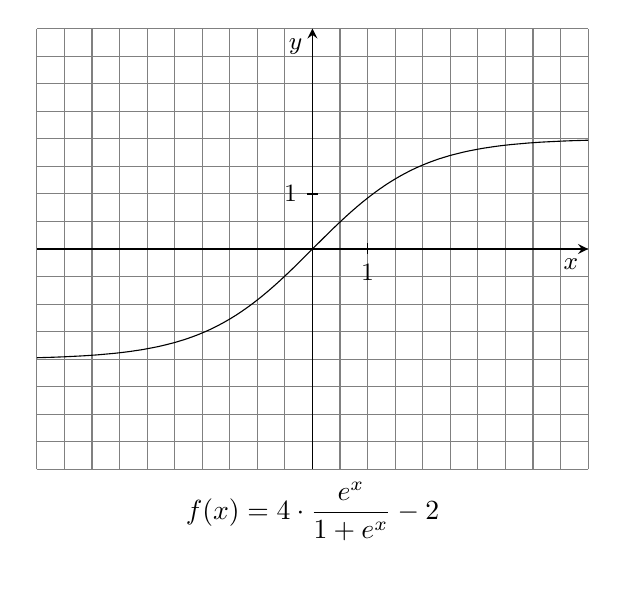
\begin{tikzpicture}[scale=0.7]
  % grid
  \draw[draw=black!50!white] (-5.000, -4.000) grid[step=0.5] (5.000, 4.000);
  % x-axis
  \draw[line width=0.6pt, ->, >=stealth] (-5.000, 0) -- (5.000, 0) node[below left] {\small$x$};
  % x scale
  \draw[line width=0.6pt] (1, 0.1) -- (1, -0.1) node[below] {\small1};
  % y-axis
  \draw[line width=0.6pt, ->, >=stealth] (0, -4.000) -- (0, 4.000) node[below left] {\small$y$};
  % y scale
  \draw[line width=0.6pt] (0.1, 1) -- (-0.1, 1) node[left] {\small1};
  % function
  \begin{scope}
    \clip (-5.000, -4.000) rectangle (5.000, 4.000);
    \draw plot[smooth] coordinates
    {
      ( -5.000,  -1.973) ( -4.900,  -1.970) ( -4.800,  -1.967)
      ( -4.700,  -1.964) ( -4.600,  -1.960) ( -4.500,  -1.956)
      ( -4.400,  -1.951) ( -4.300,  -1.946) ( -4.200,  -1.941)
      ( -4.100,  -1.935) ( -4.000,  -1.928) ( -3.900,  -1.921)
      ( -3.800,  -1.912) ( -3.700,  -1.903) ( -3.600,  -1.894)
      ( -3.500,  -1.883) ( -3.400,  -1.871) ( -3.300,  -1.858)
      ( -3.200,  -1.843) ( -3.100,  -1.828) ( -3.000,  -1.810)
      ( -2.900,  -1.791) ( -2.800,  -1.771) ( -2.700,  -1.748)
      ( -2.600,  -1.723) ( -2.500,  -1.697) ( -2.400,  -1.667)
      ( -2.300,  -1.636) ( -2.200,  -1.601) ( -2.100,  -1.564)
      ( -2.000,  -1.523) ( -1.900,  -1.480) ( -1.800,  -1.433)
      ( -1.700,  -1.382) ( -1.600,  -1.328) ( -1.500,  -1.270)
      ( -1.400,  -1.209) ( -1.300,  -1.143) ( -1.200,  -1.074)
      ( -1.100,  -1.001) ( -1.000,  -0.924) ( -0.900,  -0.844)
      ( -0.800,  -0.760) ( -0.700,  -0.673) ( -0.600,  -0.583)
      ( -0.500,  -0.490) ( -0.400,  -0.395) ( -0.300,  -0.298)
      ( -0.200,  -0.199) ( -0.100,  -0.100) (  0.000,   0.000)
      (  0.100,   0.100) (  0.200,   0.199) (  0.300,   0.298)
      (  0.400,   0.395) (  0.500,   0.490) (  0.600,   0.583)
      (  0.700,   0.673) (  0.800,   0.760) (  0.900,   0.844)
      (  1.000,   0.924) (  1.100,   1.001) (  1.200,   1.074)
      (  1.300,   1.143) (  1.400,   1.209) (  1.500,   1.270)
      (  1.600,   1.328) (  1.700,   1.382) (  1.800,   1.433)
      (  1.900,   1.480) (  2.000,   1.523) (  2.100,   1.564)
      (  2.200,   1.601) (  2.300,   1.636) (  2.400,   1.667)
      (  2.500,   1.697) (  2.600,   1.723) (  2.700,   1.748)
      (  2.800,   1.771) (  2.900,   1.791) (  3.000,   1.810)
      (  3.100,   1.828) (  3.200,   1.843) (  3.300,   1.858)
      (  3.400,   1.871) (  3.500,   1.883) (  3.600,   1.894)
      (  3.700,   1.903) (  3.800,   1.912) (  3.900,   1.921)
      (  4.000,   1.928) (  4.100,   1.935) (  4.200,   1.941)
      (  4.300,   1.946) (  4.400,   1.951) (  4.500,   1.956)
      (  4.600,   1.960) (  4.700,   1.964) (  4.800,   1.967)
      (  4.900,   1.970) (  5.000,   1.973)
    };
  \end{scope}
  \node[below] at (0.000, -4.000)
  {%
    \rule[-1.1\baselineskip]{0pt}{2.2\baselineskip}%
    \begin{minipage}{7.000cm}%
      \begin{equation*}%
        f(x)=4\cdot\frac{e^x}{1+e^x}-2
      \end{equation*}%
    \end{minipage}%
  };
\end{tikzpicture}


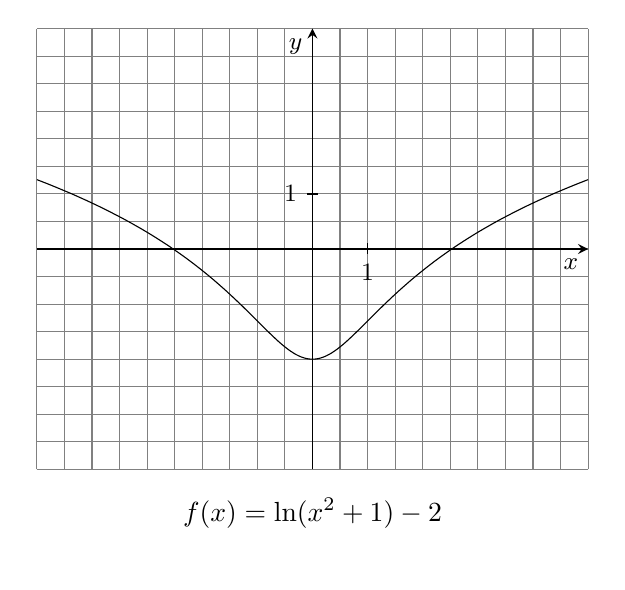
\begin{tikzpicture}[scale=0.7]
  % grid
  \draw[draw=black!50!white] (-5.000, -4.000) grid[step=0.5] (5.000, 4.000);
  % x-axis
  \draw[line width=0.6pt, ->, >=stealth] (-5.000, 0) -- (5.000, 0) node[below left] {\small$x$};
  % x scale
  \draw[line width=0.6pt] (1, 0.1) -- (1, -0.1) node[below] {\small1};
  % y-axis
  \draw[line width=0.6pt, ->, >=stealth] (0, -4.000) -- (0, 4.000) node[below left] {\small$y$};
  % y scale
  \draw[line width=0.6pt] (0.1, 1) -- (-0.1, 1) node[left] {\small1};
  % function
  \begin{scope}
    \clip (-5.000, -4.000) rectangle (5.000, 4.000);
    \draw plot[smooth] coordinates
    {
      ( -5.000,   1.258) ( -4.900,   1.219) ( -4.800,   1.180)
      ( -4.700,   1.139) ( -4.600,   1.098) ( -4.500,   1.056)
      ( -4.400,   1.014) ( -4.300,   0.970) ( -4.200,   0.925)
      ( -4.100,   0.880) ( -4.000,   0.833) ( -3.900,   0.786)
      ( -3.800,   0.737) ( -3.700,   0.687) ( -3.600,   0.636)
      ( -3.500,   0.584) ( -3.400,   0.531) ( -3.300,   0.476)
      ( -3.200,   0.419) ( -3.100,   0.362) ( -3.000,   0.303)
      ( -2.900,   0.242) ( -2.800,   0.179) ( -2.700,   0.115)
      ( -2.600,   0.049) ( -2.500,  -0.019) ( -2.400,  -0.089)
      ( -2.300,  -0.161) ( -2.200,  -0.235) ( -2.100,  -0.312)
      ( -2.000,  -0.391) ( -1.900,  -0.472) ( -1.800,  -0.555)
      ( -1.700,  -0.642) ( -1.600,  -0.730) ( -1.500,  -0.821)
      ( -1.400,  -0.915) ( -1.300,  -1.010) ( -1.200,  -1.108)
      ( -1.100,  -1.207) ( -1.000,  -1.307) ( -0.900,  -1.407)
      ( -0.800,  -1.505) ( -0.700,  -1.601) ( -0.600,  -1.693)
      ( -0.500,  -1.777) ( -0.400,  -1.852) ( -0.300,  -1.914)
      ( -0.200,  -1.961) ( -0.100,  -1.990) (  0.000,  -2.000)
      (  0.100,  -1.990) (  0.200,  -1.961) (  0.300,  -1.914)
      (  0.400,  -1.852) (  0.500,  -1.777) (  0.600,  -1.693)
      (  0.700,  -1.601) (  0.800,  -1.505) (  0.900,  -1.407)
      (  1.000,  -1.307) (  1.100,  -1.207) (  1.200,  -1.108)
      (  1.300,  -1.010) (  1.400,  -0.915) (  1.500,  -0.821)
      (  1.600,  -0.730) (  1.700,  -0.642) (  1.800,  -0.555)
      (  1.900,  -0.472) (  2.000,  -0.391) (  2.100,  -0.312)
      (  2.200,  -0.235) (  2.300,  -0.161) (  2.400,  -0.089)
      (  2.500,  -0.019) (  2.600,   0.049) (  2.700,   0.115)
      (  2.800,   0.179) (  2.900,   0.242) (  3.000,   0.303)
      (  3.100,   0.362) (  3.200,   0.419) (  3.300,   0.476)
      (  3.400,   0.531) (  3.500,   0.584) (  3.600,   0.636)
      (  3.700,   0.687) (  3.800,   0.737) (  3.900,   0.786)
      (  4.000,   0.833) (  4.100,   0.880) (  4.200,   0.925)
      (  4.300,   0.970) (  4.400,   1.014) (  4.500,   1.056)
      (  4.600,   1.098) (  4.700,   1.139) (  4.800,   1.180)
      (  4.900,   1.219) (  5.000,   1.258)
    };
  \end{scope}
  \node[below] at (0.000, -4.000)
  {%
    \rule[-1.1\baselineskip]{0pt}{2.2\baselineskip}%
    \begin{minipage}{7.000cm}%
      \begin{equation*}%
        f(x)=\ln(x^2+1)-2
      \end{equation*}%
    \end{minipage}%
  };
\end{tikzpicture}

\hfill
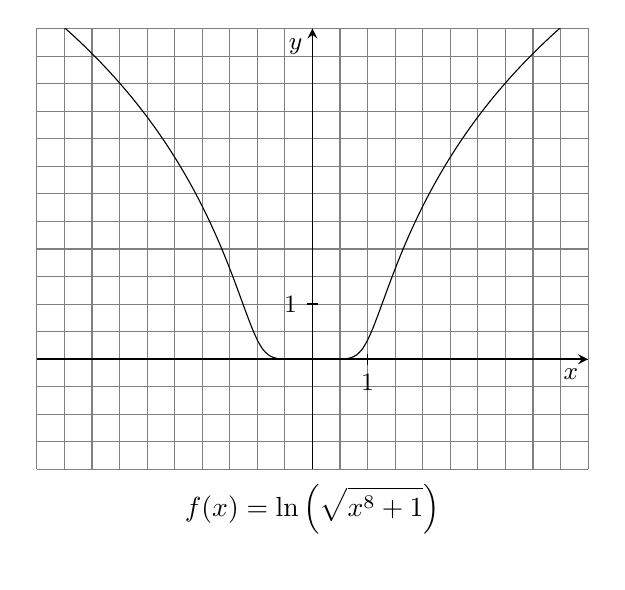
\begin{tikzpicture}[scale=0.7]
  % grid
  \draw[draw=black!50!white] (-5.000, -2.000) grid[step=0.5] (5.000, 6.000);
  % x-axis
  \draw[line width=0.6pt, ->, >=stealth] (-5.000, 0) -- (5.000, 0) node[below left] {\small$x$};
  % x scale
  \draw[line width=0.6pt] (1, 0.1) -- (1, -0.1) node[below] {\small1};
  % y-axis
  \draw[line width=0.6pt, ->, >=stealth] (0, -2.000) -- (0, 6.000) node[below left] {\small$y$};
  % y scale
  \draw[line width=0.6pt] (0.1, 1) -- (-0.1, 1) node[left] {\small1};
  % function
  \begin{scope}
    \clip (-5.000, -2.000) rectangle (5.000, 6.000);
    \draw plot[smooth] coordinates
    {
      ( -5.000,   6.438) ( -4.900,   6.357) ( -4.800,   6.274)
      ( -4.700,   6.190) ( -4.600,   6.104) ( -4.500,   6.016)
      ( -4.400,   5.926) ( -4.300,   5.834) ( -4.200,   5.740)
      ( -4.100,   5.644) ( -4.000,   5.545) ( -3.900,   5.444)
      ( -3.800,   5.340) ( -3.700,   5.233) ( -3.600,   5.124)
      ( -3.500,   5.011) ( -3.400,   4.895) ( -3.300,   4.776)
      ( -3.200,   4.653) ( -3.100,   4.526) ( -3.000,   4.395)
      ( -2.900,   4.259) ( -2.800,   4.119) ( -2.700,   3.973)
      ( -2.600,   3.822) ( -2.500,   3.665) ( -2.400,   3.502)
      ( -2.300,   3.332) ( -2.200,   3.155) ( -2.100,   2.969)
      ( -2.000,   2.775) ( -1.900,   2.570) ( -1.800,   2.356)
      ( -1.700,   2.130) ( -1.600,   1.892) ( -1.500,   1.641)
      ( -1.400,   1.379) ( -1.300,   1.107) ( -1.200,   0.834)
      ( -1.100,   0.573) ( -1.000,   0.347) ( -0.900,   0.179)
      ( -0.800,   0.078) ( -0.700,   0.028) ( -0.600,   0.008)
      ( -0.500,   0.002) ( -0.400,   0.000) ( -0.300,   0.000)
      ( -0.200,   0.000) ( -0.100,   0.000) (  0.000,   0.000)
      (  0.100,   0.000) (  0.200,   0.000) (  0.300,   0.000)
      (  0.400,   0.000) (  0.500,   0.002) (  0.600,   0.008)
      (  0.700,   0.028) (  0.800,   0.078) (  0.900,   0.179)
      (  1.000,   0.347) (  1.100,   0.573) (  1.200,   0.834)
      (  1.300,   1.107) (  1.400,   1.379) (  1.500,   1.641)
      (  1.600,   1.892) (  1.700,   2.130) (  1.800,   2.356)
      (  1.900,   2.570) (  2.000,   2.775) (  2.100,   2.969)
      (  2.200,   3.155) (  2.300,   3.332) (  2.400,   3.502)
      (  2.500,   3.665) (  2.600,   3.822) (  2.700,   3.973)
      (  2.800,   4.119) (  2.900,   4.259) (  3.000,   4.395)
      (  3.100,   4.526) (  3.200,   4.653) (  3.300,   4.776)
      (  3.400,   4.895) (  3.500,   5.011) (  3.600,   5.124)
      (  3.700,   5.233) (  3.800,   5.340) (  3.900,   5.444)
      (  4.000,   5.545) (  4.100,   5.644) (  4.200,   5.740)
      (  4.300,   5.834) (  4.400,   5.926) (  4.500,   6.016)
      (  4.600,   6.104) (  4.700,   6.190) (  4.800,   6.274)
      (  4.900,   6.357) (  5.000,   6.438)
    };
  \end{scope}
  \node[below] at (0.000, -2.000)
  {%
    \rule[-1.1\baselineskip]{0pt}{2.2\baselineskip}%
    \begin{minipage}{7.000cm}%
      \begin{equation*}%
        f(x)=\ln\left(\sqrt{x^8+1}\right)
      \end{equation*}%
    \end{minipage}%
  };
\end{tikzpicture}


% ------------------------------------------------------------------------------
\end{document}
% ------------------------------------------------------------------------------
